\documentclass{article}

\usepackage[T1]{fontenc}    %Schriftart des Dokumentes
\usepackage[ngerman]{babel} %Dokumentensprache, hier Deutsch
\usepackage{amsmath, amssymb, stmaryrd} %mathematische Schriftzeichen
\usepackage{graphicx} %Einfügen von Grafiken
\usepackage{wrapfig}
\usepackage{bm}
\usepackage{subfig}
\usepackage{newclude}
\usepackage{pdfpages}
\usepackage{hyperref}
\hypersetup{
    colorlinks,
    citecolor=black,
    filecolor=black,
    linkcolor=black,
    urlcolor=black
}
\usepackage[bottom]{footmisc}

\makeatletter
\newcommand\invisiblesection[1]{%
  \refstepcounter{section}%
  \addcontentsline{toc}{section}{\protect\numberline{\thesection}#1}%
  \sectionmark{#1}\phantom{}}
\makeatother

\setlength{\parindent}{0pt} %Einrückung von Absätzen auf null gesetzt
\setlength{\parskip}{10pt} %Abstand zischen Absätzen auf 10pt gesetzt

\title{Versuch 245: Induktion}
\author{Matthias Kuntz}
\date{10.06.2024}

\renewcommand*\contentsname{Zusammenfassung}

\begin{document}

\maketitle

\tableofcontents

\newpage

%-------------------------EINLEITUNG-------------------------
\section{Einleitung}

In diesem Versuch sollen die Grundlagen der Induktion anhand der Helmholtz-Spule erarbeitet werden. Dazu betrachten wir zunächst eine in der Helmholtz-Spule angebrachte Sekundärspule, welche sich rotieren lässt und in welcher durch das Magnetfeld der primären Helmholtz-Spule eine Spannung induziert werden soll. Ebenso wollen wir mit dieser Konfiguration das Erdmagnetfeld untersuchen, wobei wir auf die Begriffe der Inklination sowie die Aufteilung in vertikale und horizontale Komponenten eingehen werden. 


\subsection{Physikalische Grundlagen}

\subsubsection{Helmholtz-Spule}

Eine Helmholtz-Spule ist eine Anordnung von zwei kurzen Spulen mit gleichem Radius $r$ und gleicher Windungszahl $N$, die parallel genau im Abstand $d = r$ parallel zueinander aufgestellt werden. Werden diese dann gleichsinnig von einem  Strom mit der Stärke $I$ durchflossen, so entsteht ein annähernd homogenes Magnetfeld zwischen den Spulen, siehe Abbildung \ref{fig:Helmholtz-Spule}, und es ergibt sich die folgende Form für den Betrag des magnetischen Felds $B$:

\begin{equation}
    B = \mu_0 \frac{8N}{\sqrt{125} r} I.
    \label{eq:Magnetfeld_THEO}
\end{equation}

Bringt man eine sich mit der Kreisfrequenz $\omega$ rotierende Flachspule zwischen die Spulen der Helmholtz-Anordnung, so wird in dieser eine Spannung induziert, sobald Strom durch die Helmholtz-Spulen fließt und das Magnetfeld zwischen diesen erzeugt wird. Für den in unserer Flachspule induzierten Strom $U_I$ gilt bei konstantem B-Feld das Induktionsgesetz

\begin{equation}
    U_I (t) = - N \frac{d \Phi}{dt} = - B A N \omega \sin{wt},
    \label{eq:Induktionsgesetz_Helmholtz}
\end{equation}

wobei $\Phi$ den magnetischen Fluss durch die Spule in Abhängigkeit der Magnetfeldstärke $B$ sowie der Fläche der Spule $A$ beschreibt. 

Fließt hingegen ein Wechselstrom der Kreisfrequenz $\Omega$ durch die Helmholtz-Spule, so entsteht ein sich änderndes Magnetfeld. Lässt man die Flachspule nun in der Helmholtz-Spule ruhen, so gilt:

\begin{equation}
    U_I = U_m \sin{\Omega t} = BAN \Omega \cos{\alpha} \sin{\Omega t}.
    \label{eq:Induktionsgesetz_Helmholtz_AC}
\end{equation}

Hierbei bezeichnet $\alpha$ den Winkel zwischen der Flachspule und dem Magnetfeld. 

Ebenso lässt sich dann die Induktivität $L$ der Helmholtz-Spule bestimmen. Diese ist mit dem gemessenen Widerstand $R$ der Spulen wie folgt verbunden:

\begin{equation}
    L = \frac{R}{\Omega} = \frac{R}{2 \pi f}.
    \label{eq:Induktivität}
\end{equation}

\begin{figure}[!b]
    \centering
    \resizebox{0.5\textwidth}{!}{
    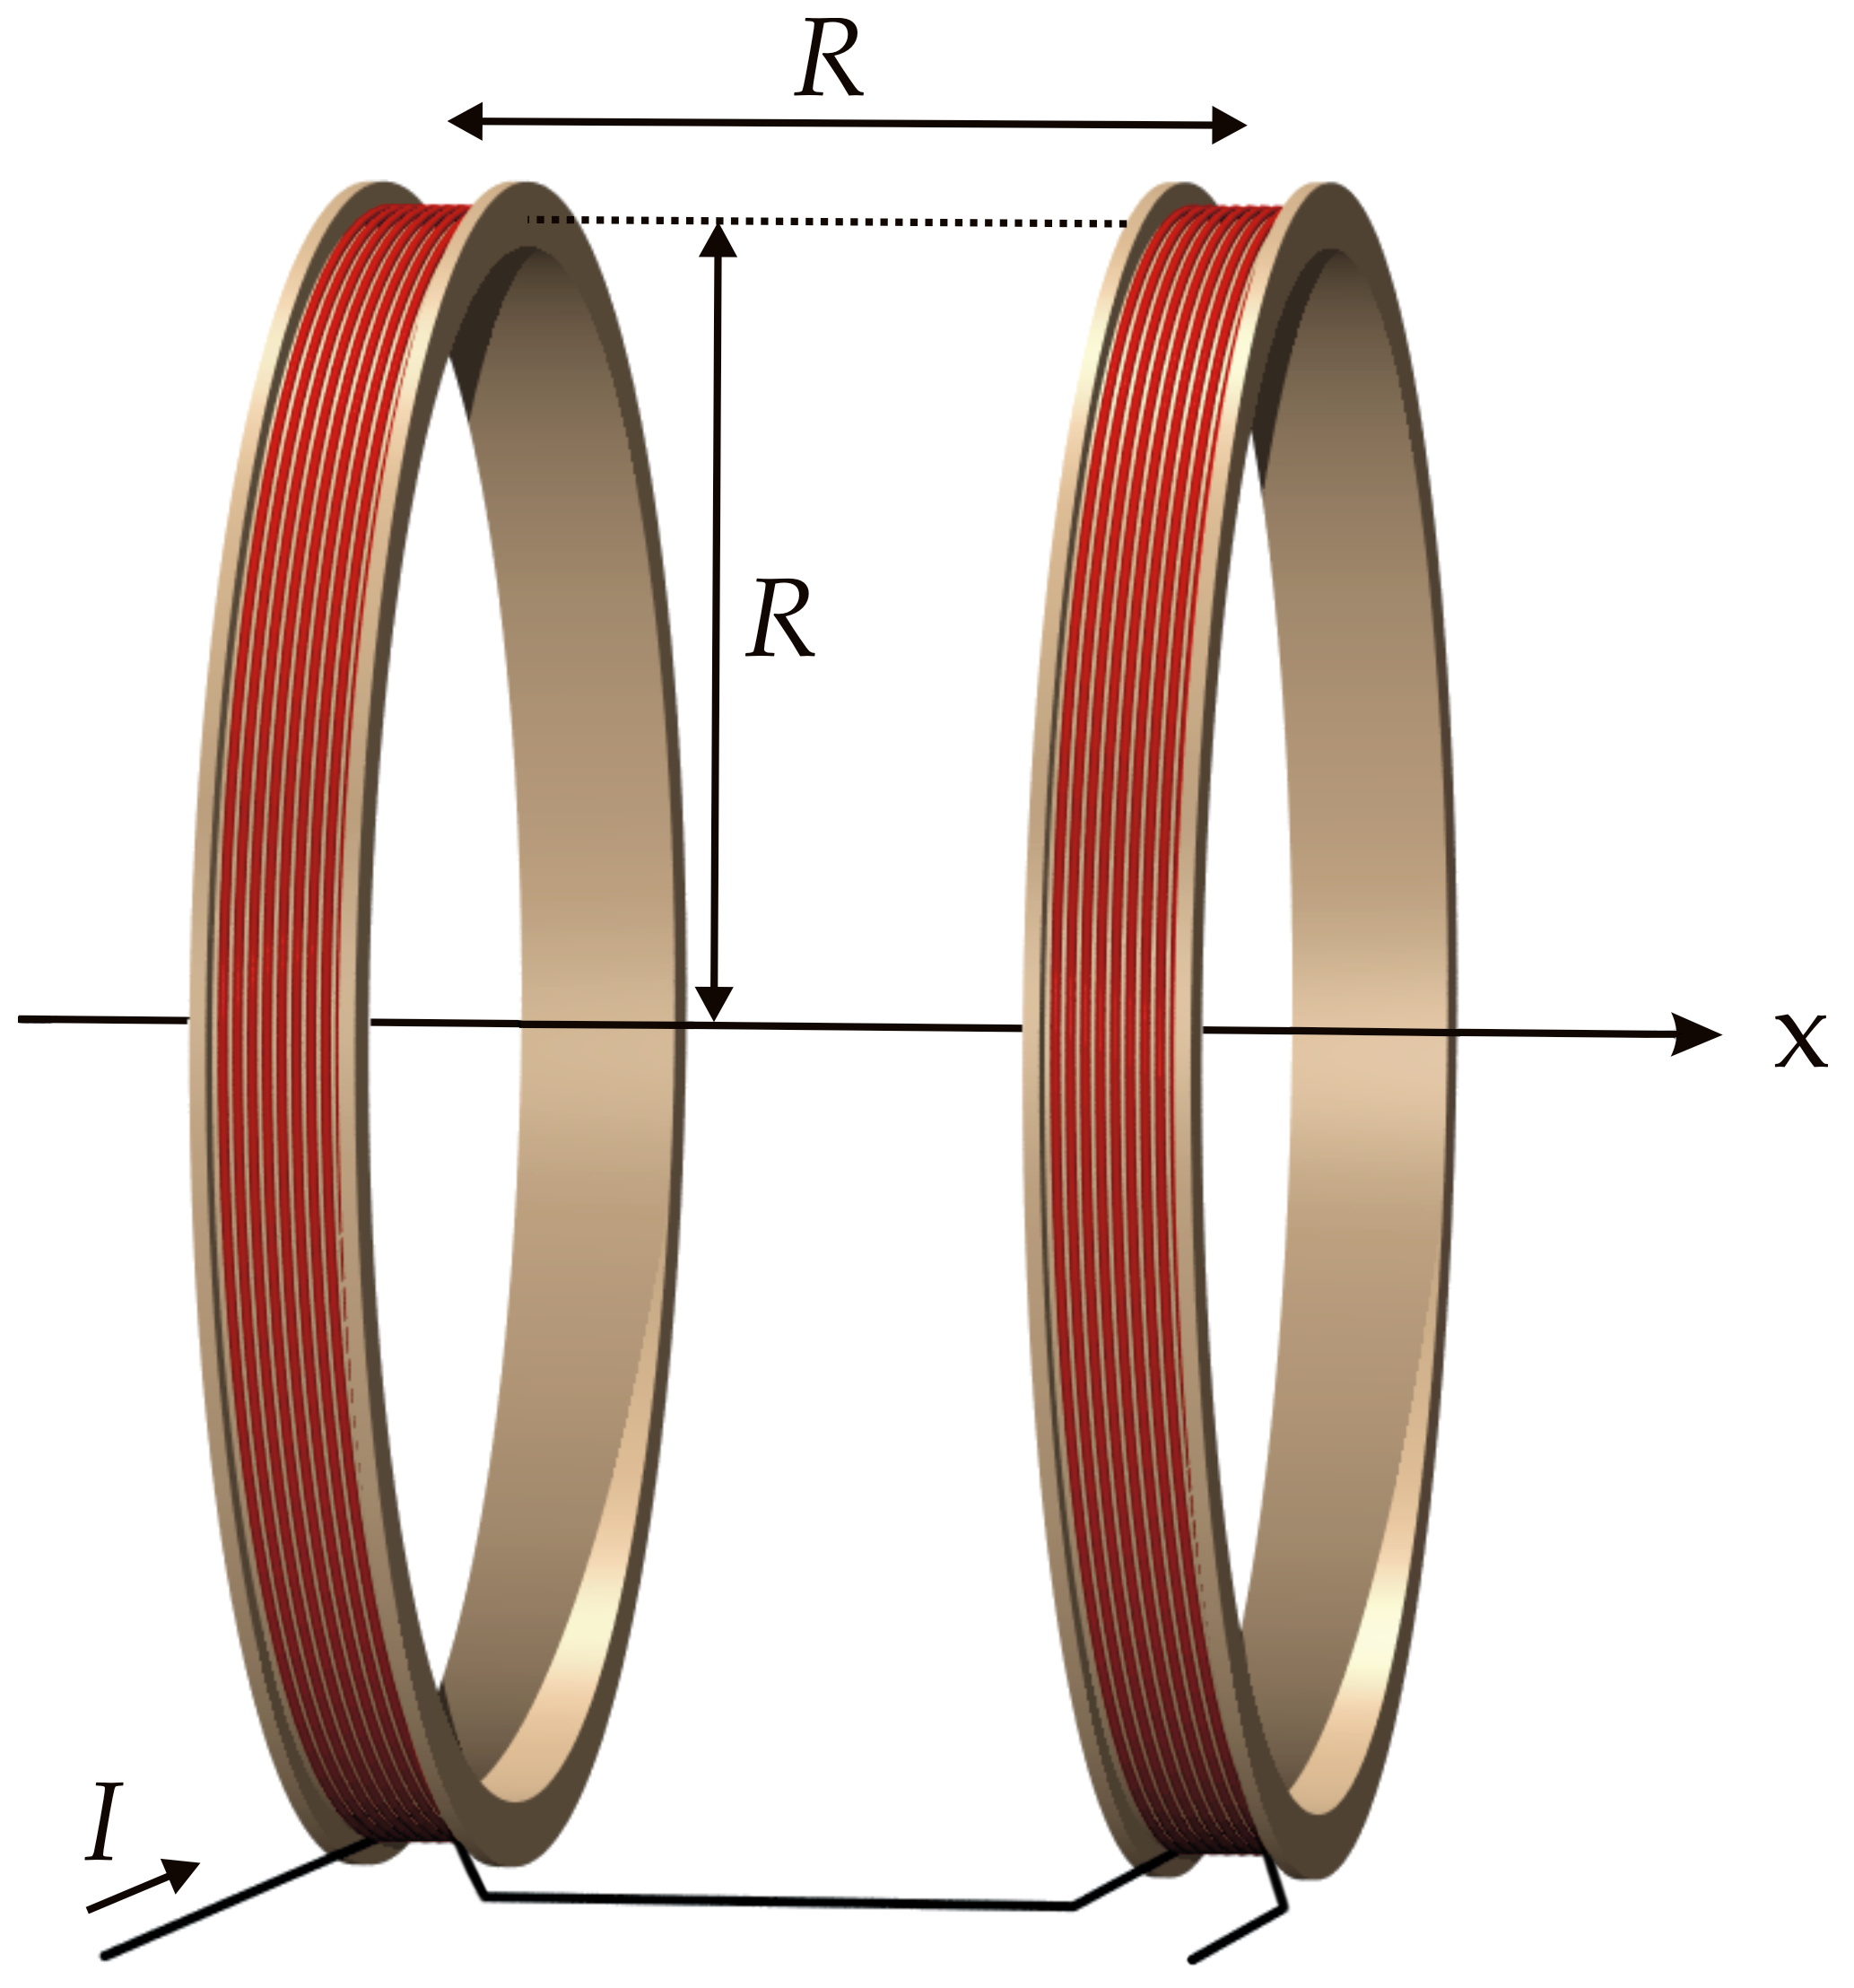
\includegraphics{graphics/Helmholtz_coils.png}}
    \caption[Helmholtz-Spule]{Helmholtz-Spule [Quelle: Ansgar Hellwig\protect\footnotemark, Stand: 04.07.2024]}
    \label{fig:Helmholtz-Spule}
\end{figure}

\footnotetext{Ansgar Hellwig, via Wikimedia Commons <\url{https://commons.wikimedia.org/wiki/File:Helmholtz_coils.png}>}

\newpage
\subsubsection{Erdmagnetfeld}

Das Erdmagnetfeld lässt sich als großes die Erde umgebendes Magnetfeld annähern, das durch einen Stabmagneten erzeugt wird, der einmal quer durch die Erde verläuft, siehe Abbildung \ref{fig:erdmagnetfeld}a. Dabei verlaufen nur in der Nähe des Äquators die Feldlinien annähernd parallel zur Erdoberfläche und treffen an anderen Positionen unter einem Inklinationswinkel $i$ auf die Erdoberfläche, Abbildung \ref{fig:erdmagnetfeld}c. Somit kann man das Erdmagnetfeld aufteilen in einen horizontalen und vertikalen Anteil $B_H$ \& $B_V$:

\begin{equation}
        \cos{i} = \frac{B_H}{B}, \ \ \  \sin{i} = \frac{B_V}{B}.
        \label{eq:Inklination}
\end{equation}

Gemäß der ZAMG\footnotemark betrugen das Erdmagnetfeld und die Deklination zum Tag des Versuchs in Heidelberg:

\footnotetext{ZAMG Website, IGRF Deklinationsrechner <\url{https://www.zamg.ac.at/cms/de/geophysik/produkte-und-services-1/online-deklinationsrechner}>}

\begin{equation}
    \begin{split}
        B &= 48909,8 \cdot 10^{-9} \text{T} \\
        i &= 65,2^\circ
    \end{split}
    \label{eq:Erdmagnetfeld-Theo}
\end{equation}


\begin{figure}[!h]
    \centering
    \resizebox{0.6\textwidth}{!}{
    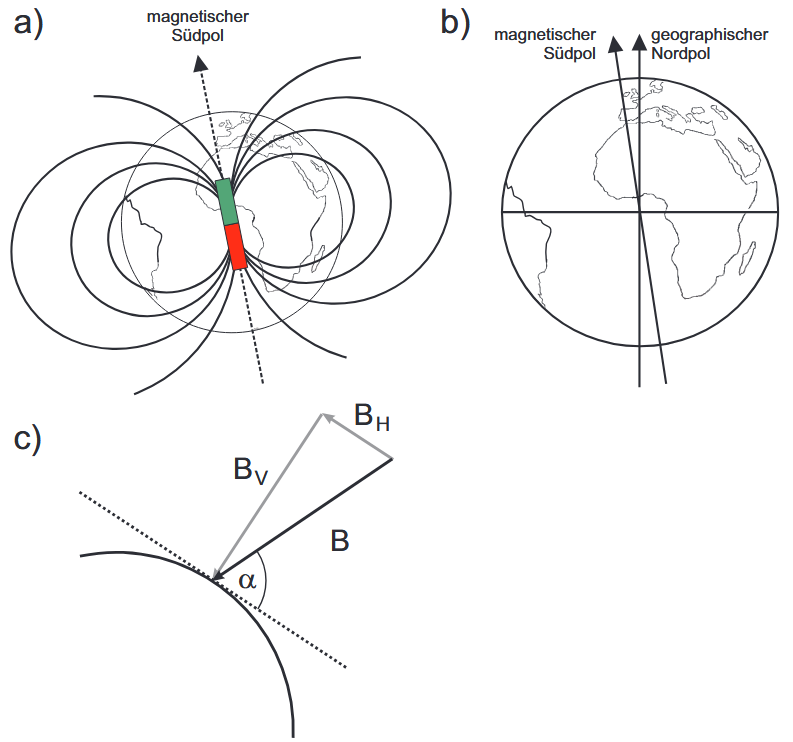
\includegraphics{graphics/erdmagnetfeld.png}}
    \caption{Erdmagnetfeld: a) Schematischer Verlauf, b) Abweichung von den geografischen Polen, c) Zerlegung in Komponenten [Quelle: PAP2.2 Skript, S.49, Stand: 29.07.2024]}
    \label{fig:Erdmagnetfeld}
\end{figure}

\newpage
\subsection{Versuchsaufbau}

Herzstück des in Abbildung \ref{fig:Aufbau} dargestellten Aufbaus ist die Helmholtz-Spule (Durchmesser $295$mm, Abstand der Spulen $147$mm, Windungszahl je Spule 124) mit eingebauter drehbarer Sekundärspule (Windungszahl 4000, Fläche 41,7 cm$^2$), welche über einen Riemen mit dem Antriebsmotor verbunden ist. Der Strom durch die Helmholtz-Spule wird von einem Leistungsfunktionsgenerator geliefert und die induzierte Spannung in der Sekundärspule von einem Oszilloskop gemessen. Zusätzlich werden Multimeter zur gleichzeitigen Strommessung verwendet.  

\begin{figure}[!b]
    \centering
    \resizebox{0.9\textwidth}{!}{
    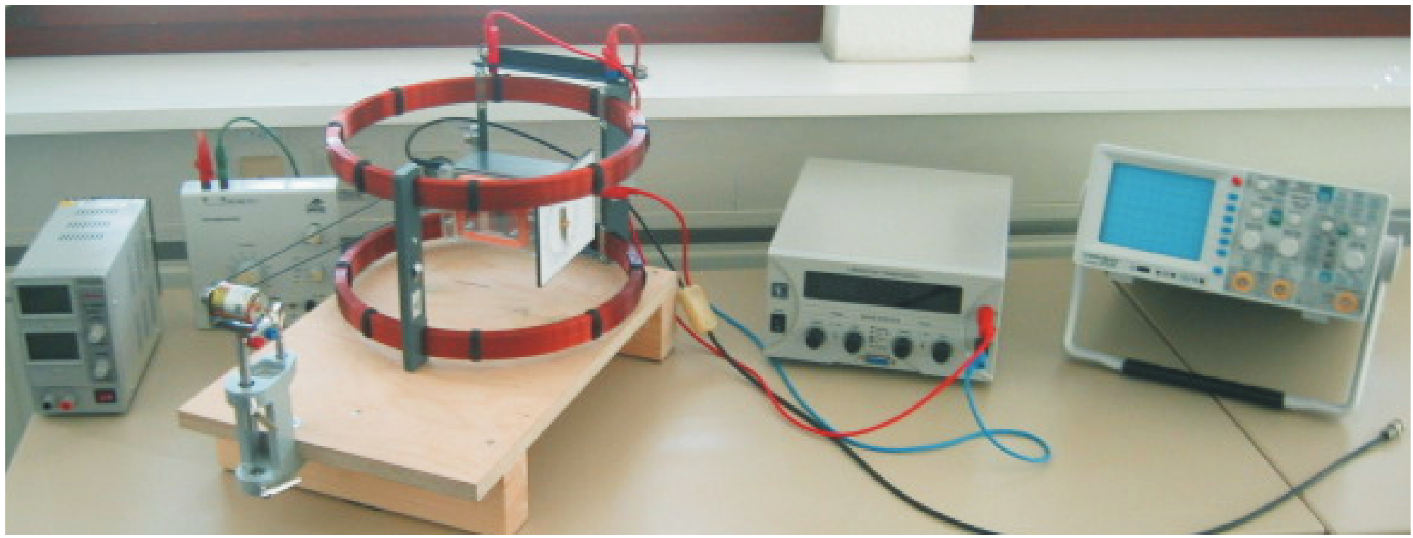
\includegraphics{graphics/aufbau.png}}
    \caption{Versuchsaufbau [Quelle: PAP2.2 Skript, S.46, Stand: 30.07.2024]}
    \label{fig:Aufbau}
\end{figure}


\phantom{.}





%---------------VERSUCHSPROTOKOLL MIT MESSDATEN---------------
\newpage

\section{Versuchsprotokoll mit Messdaten}

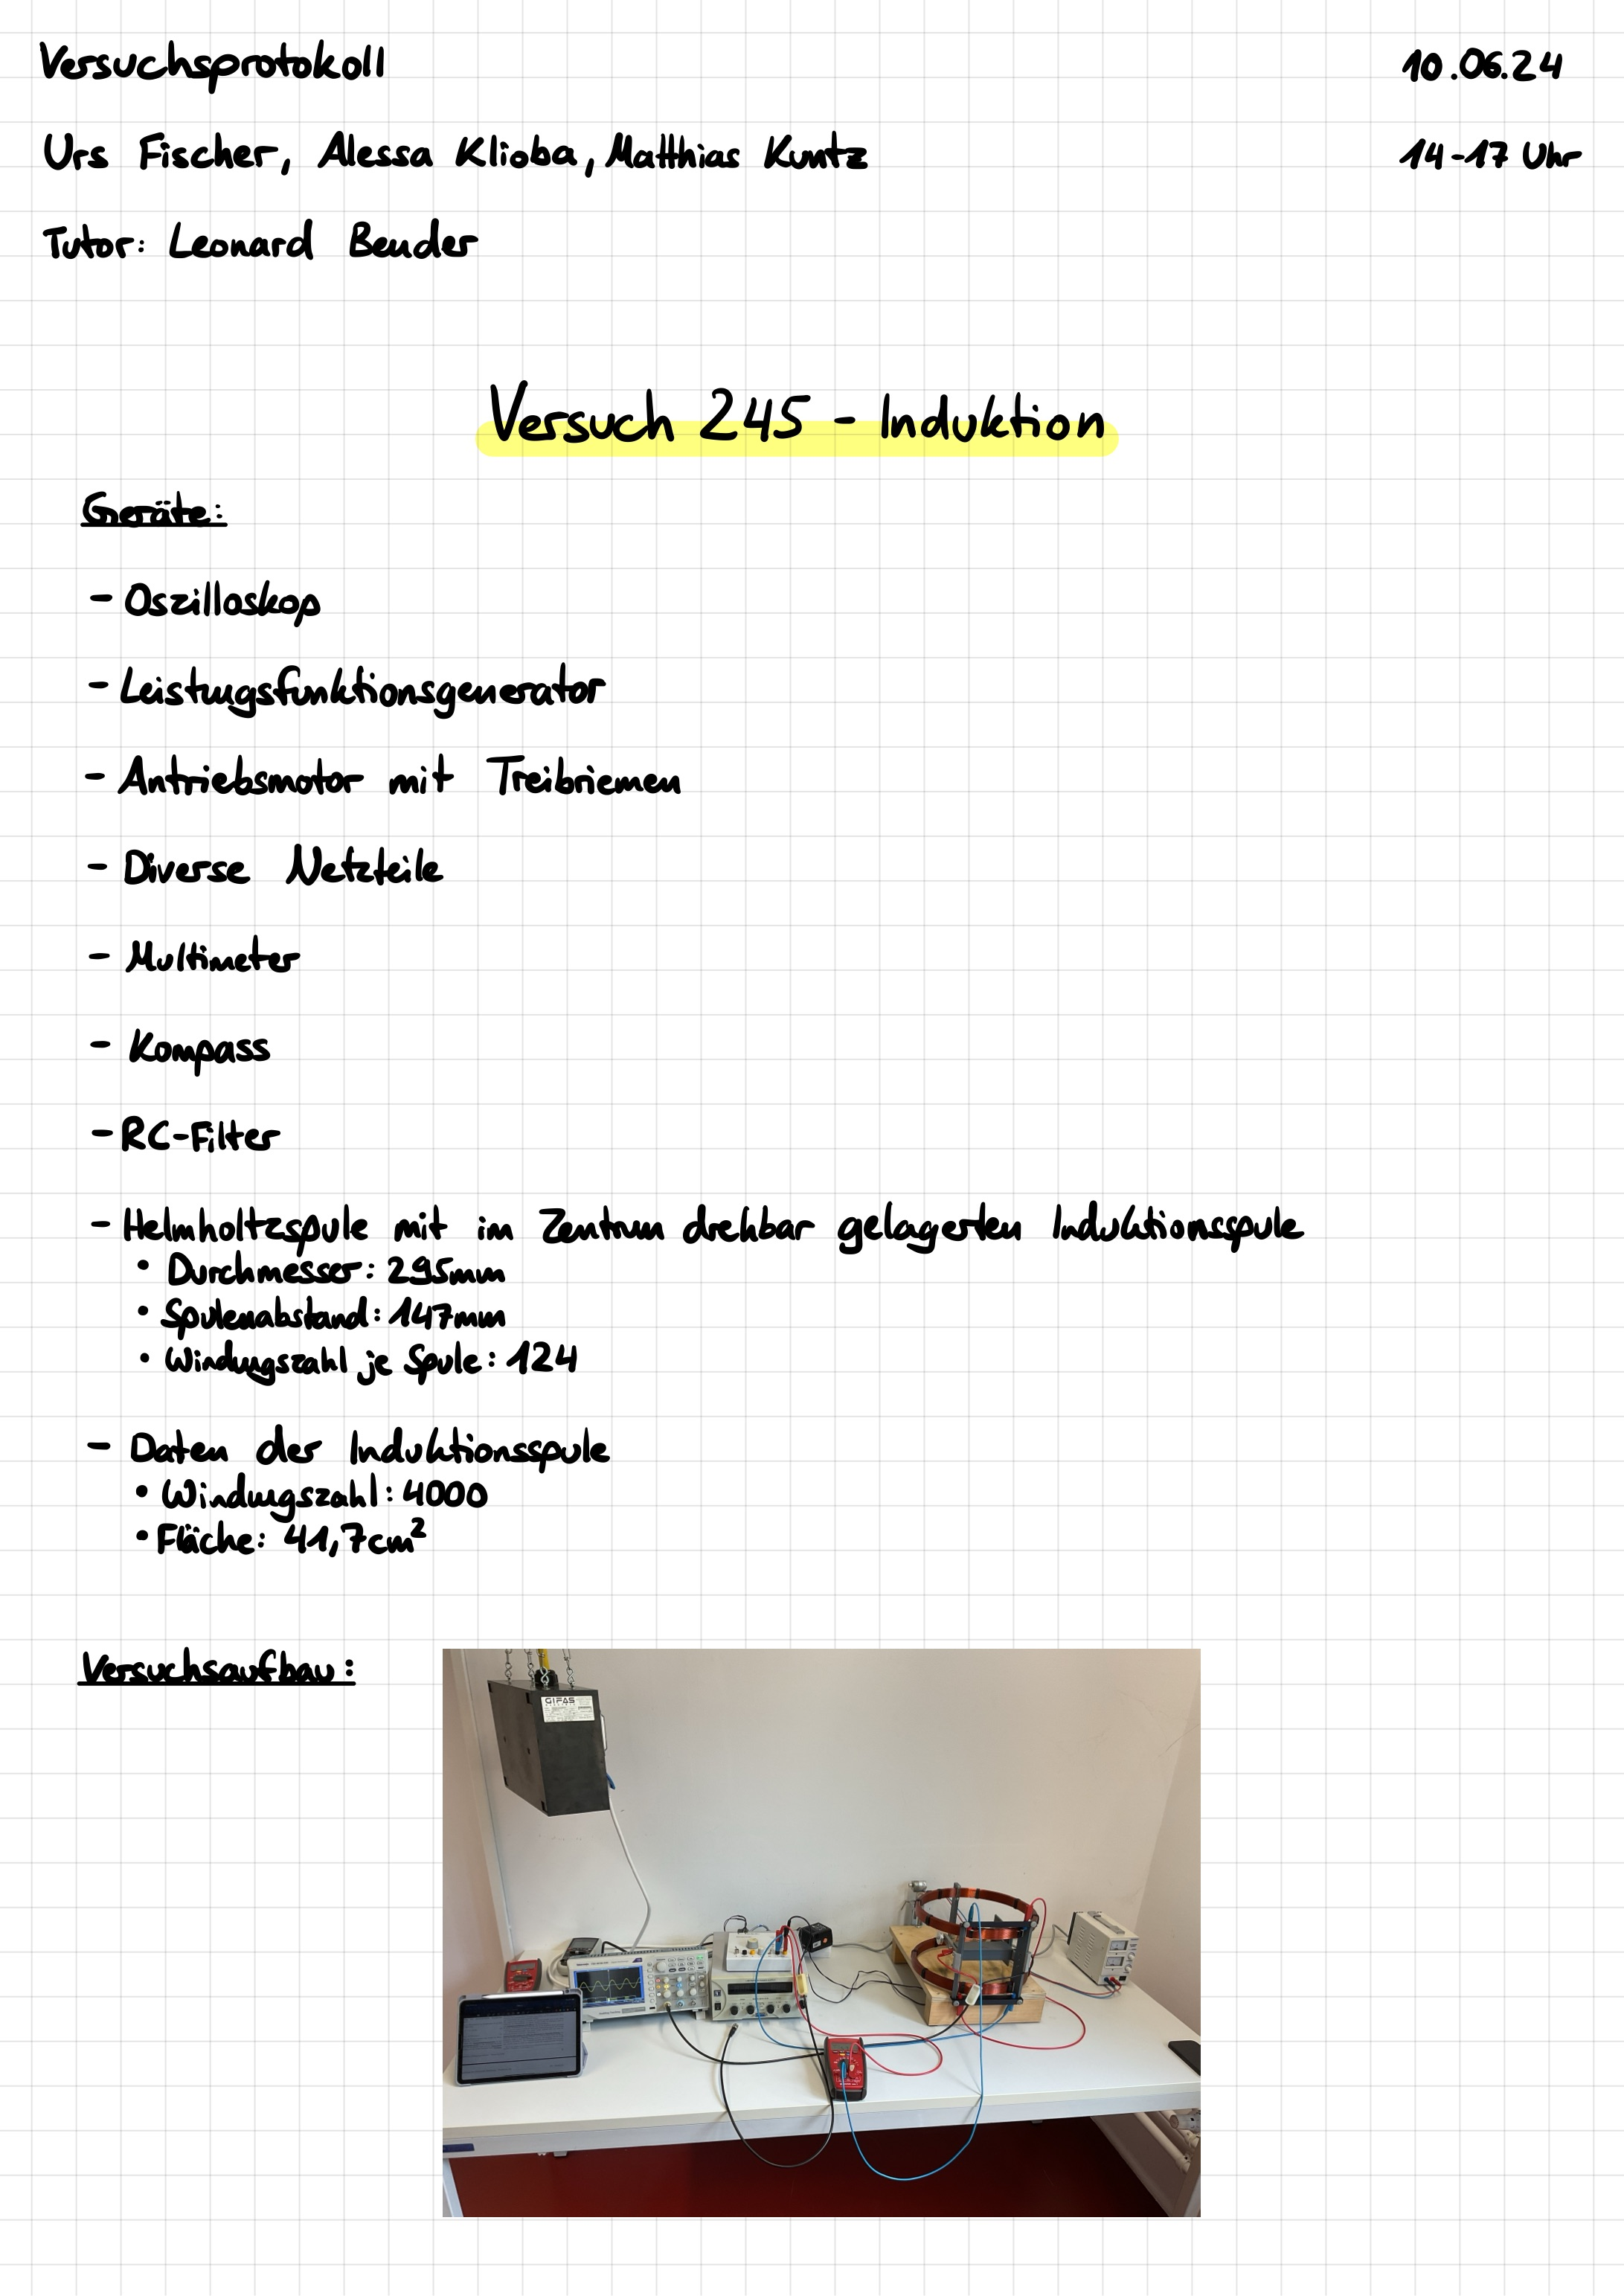
\includegraphics[width=\textwidth]{graphics/mess1.jpg}
\newpage
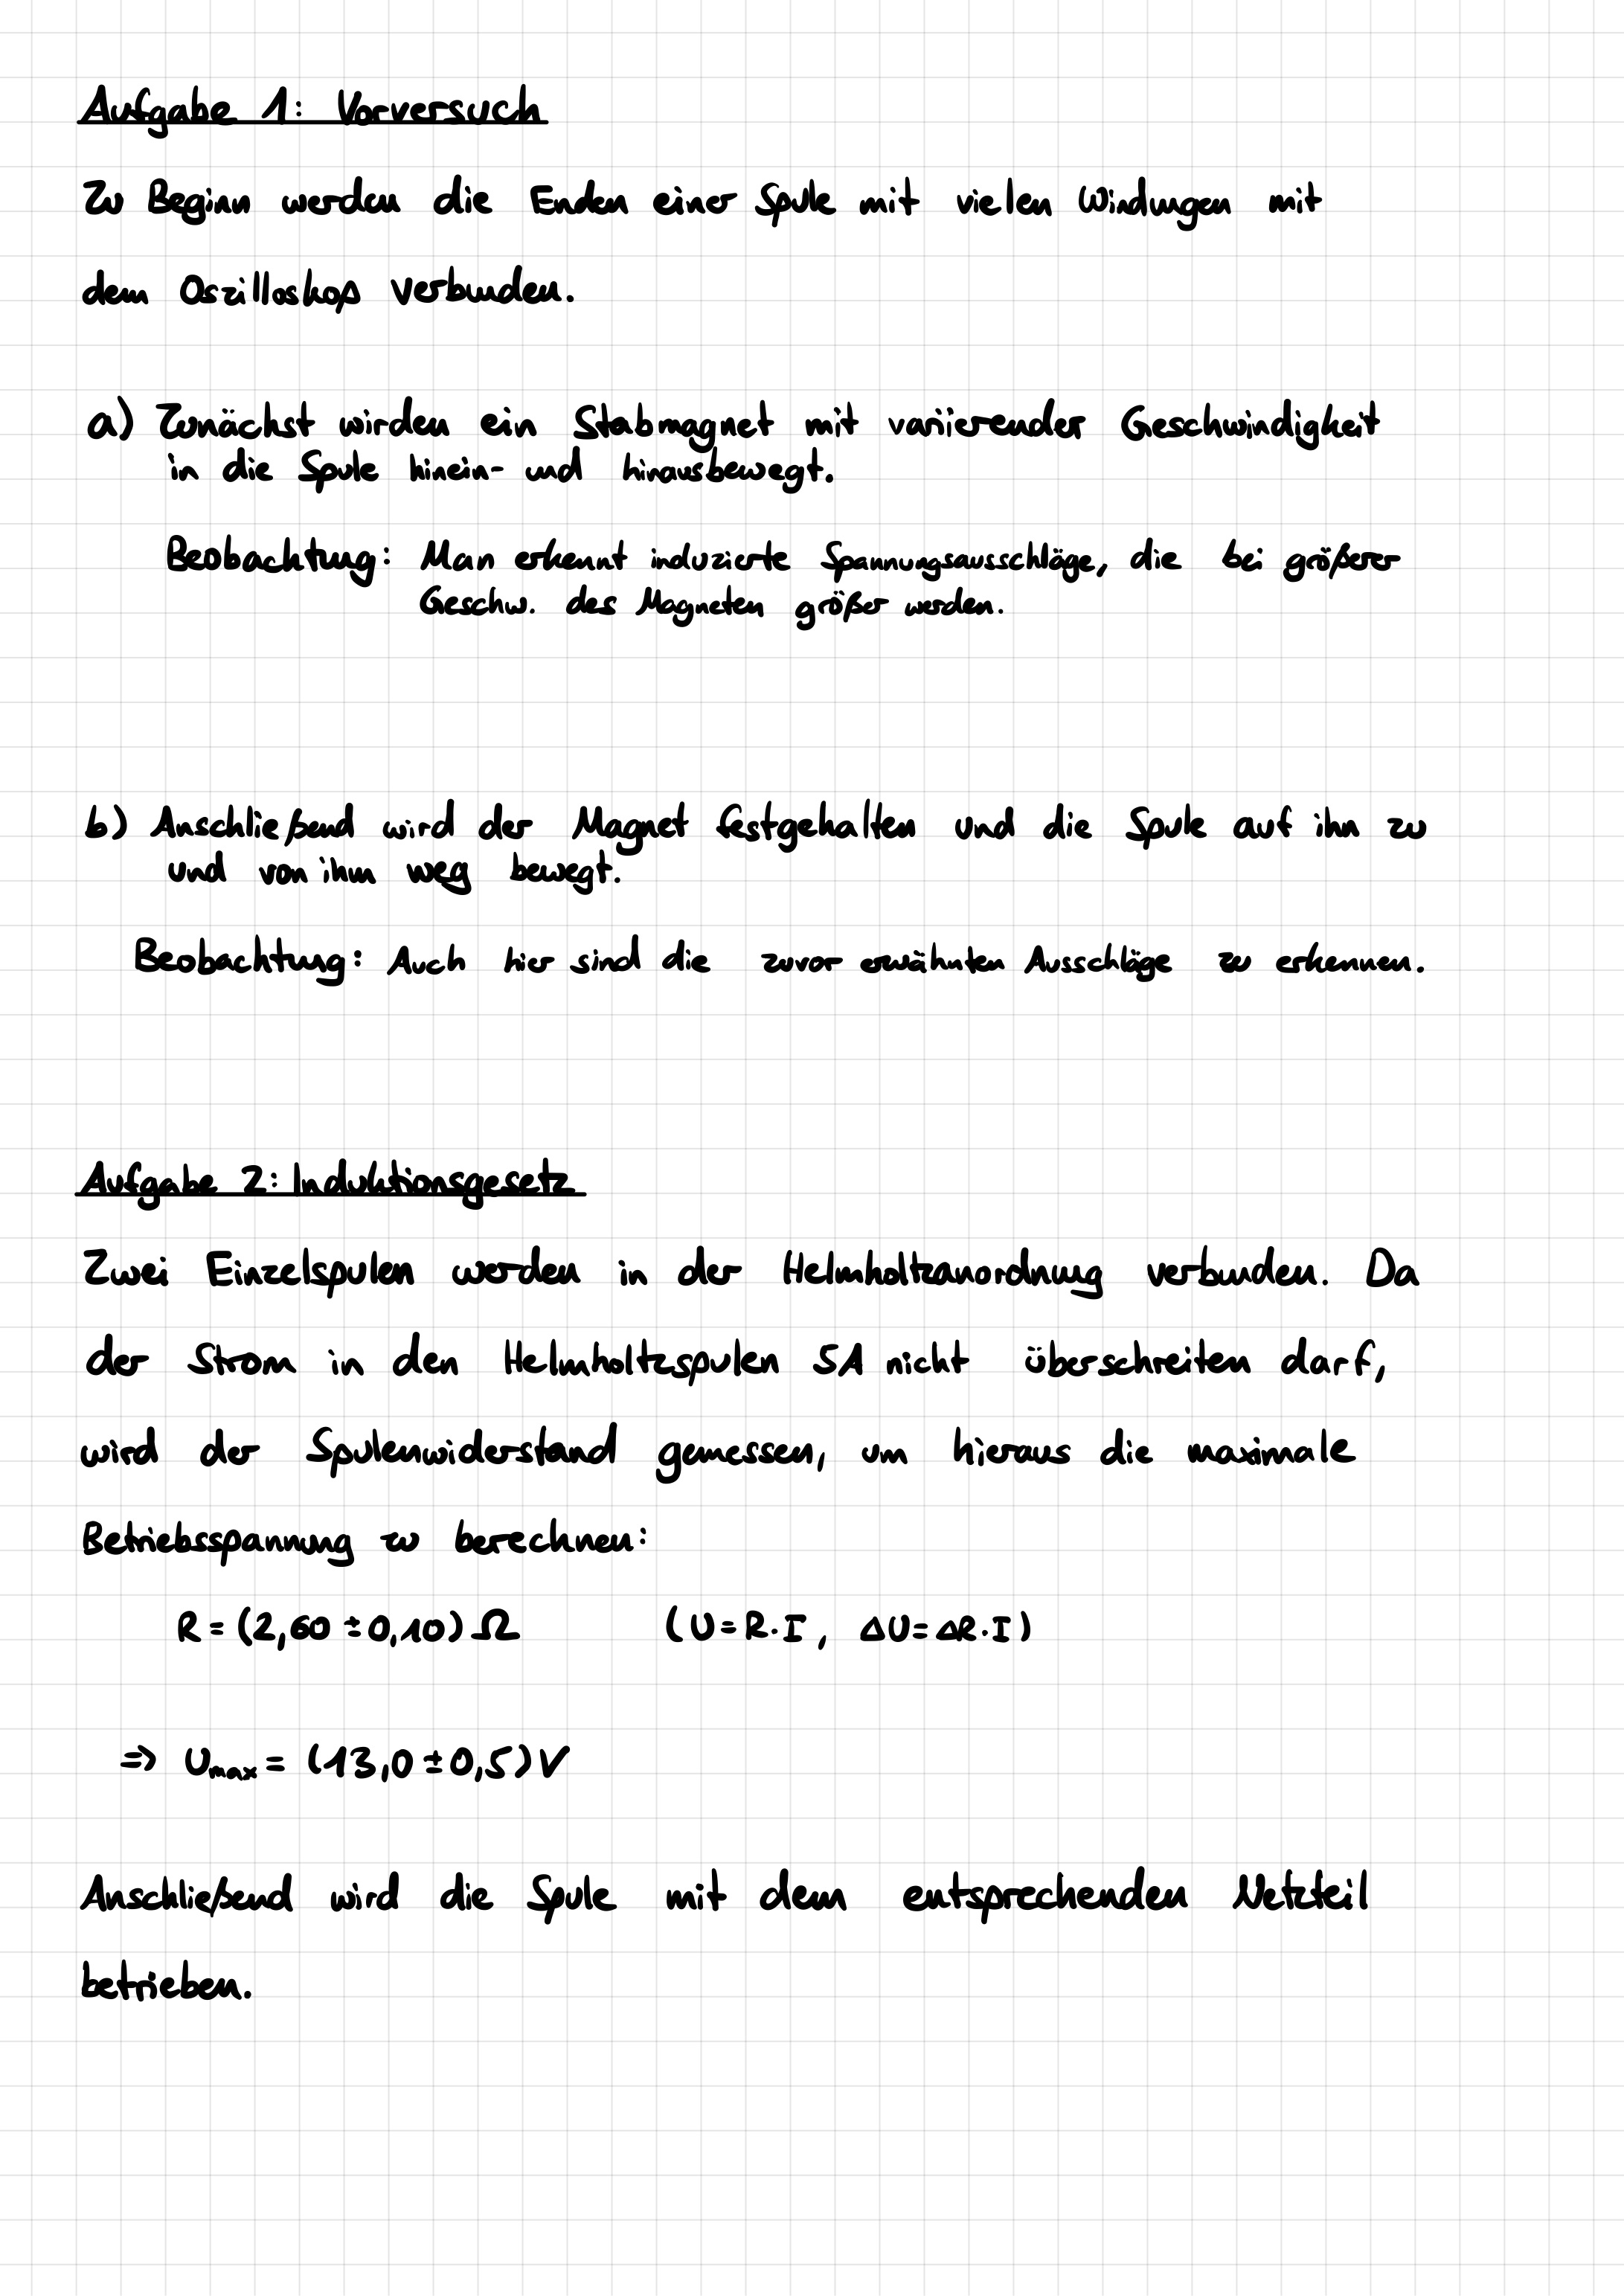
\includegraphics[width=\textwidth]{graphics/mess2.jpg}
\newpage
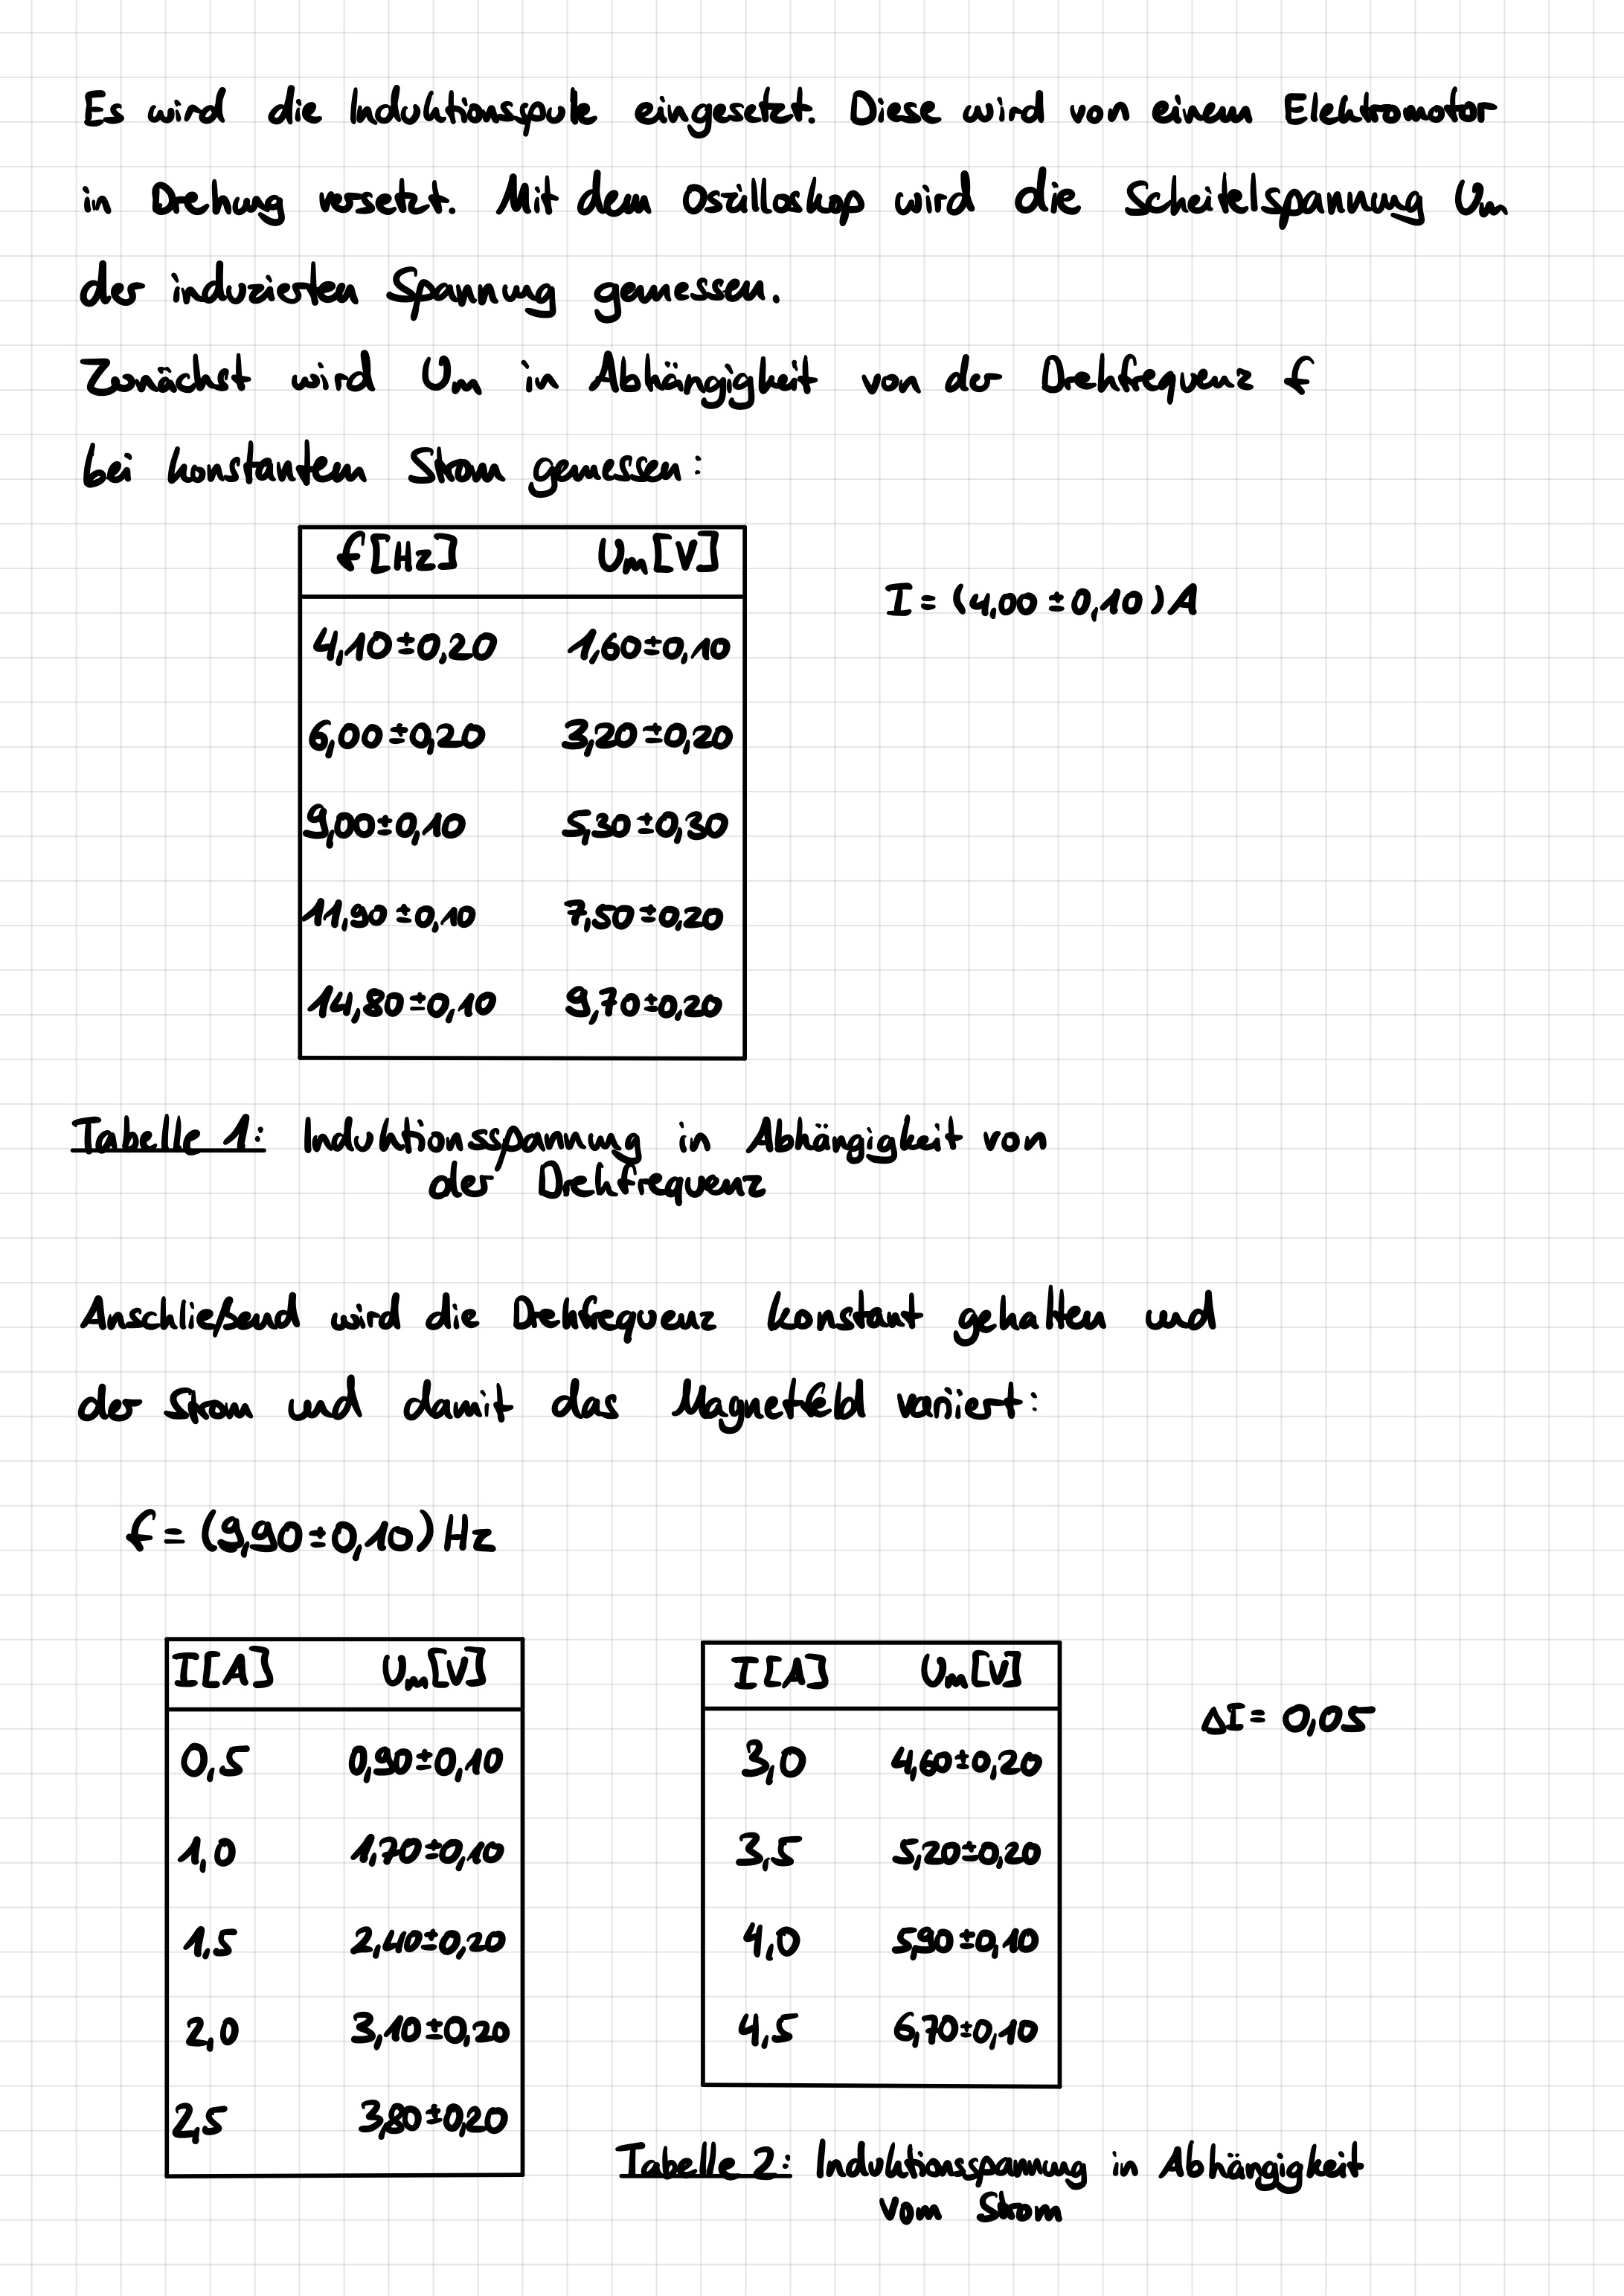
\includegraphics[width=\textwidth]{graphics/mess3.jpg}
\newpage
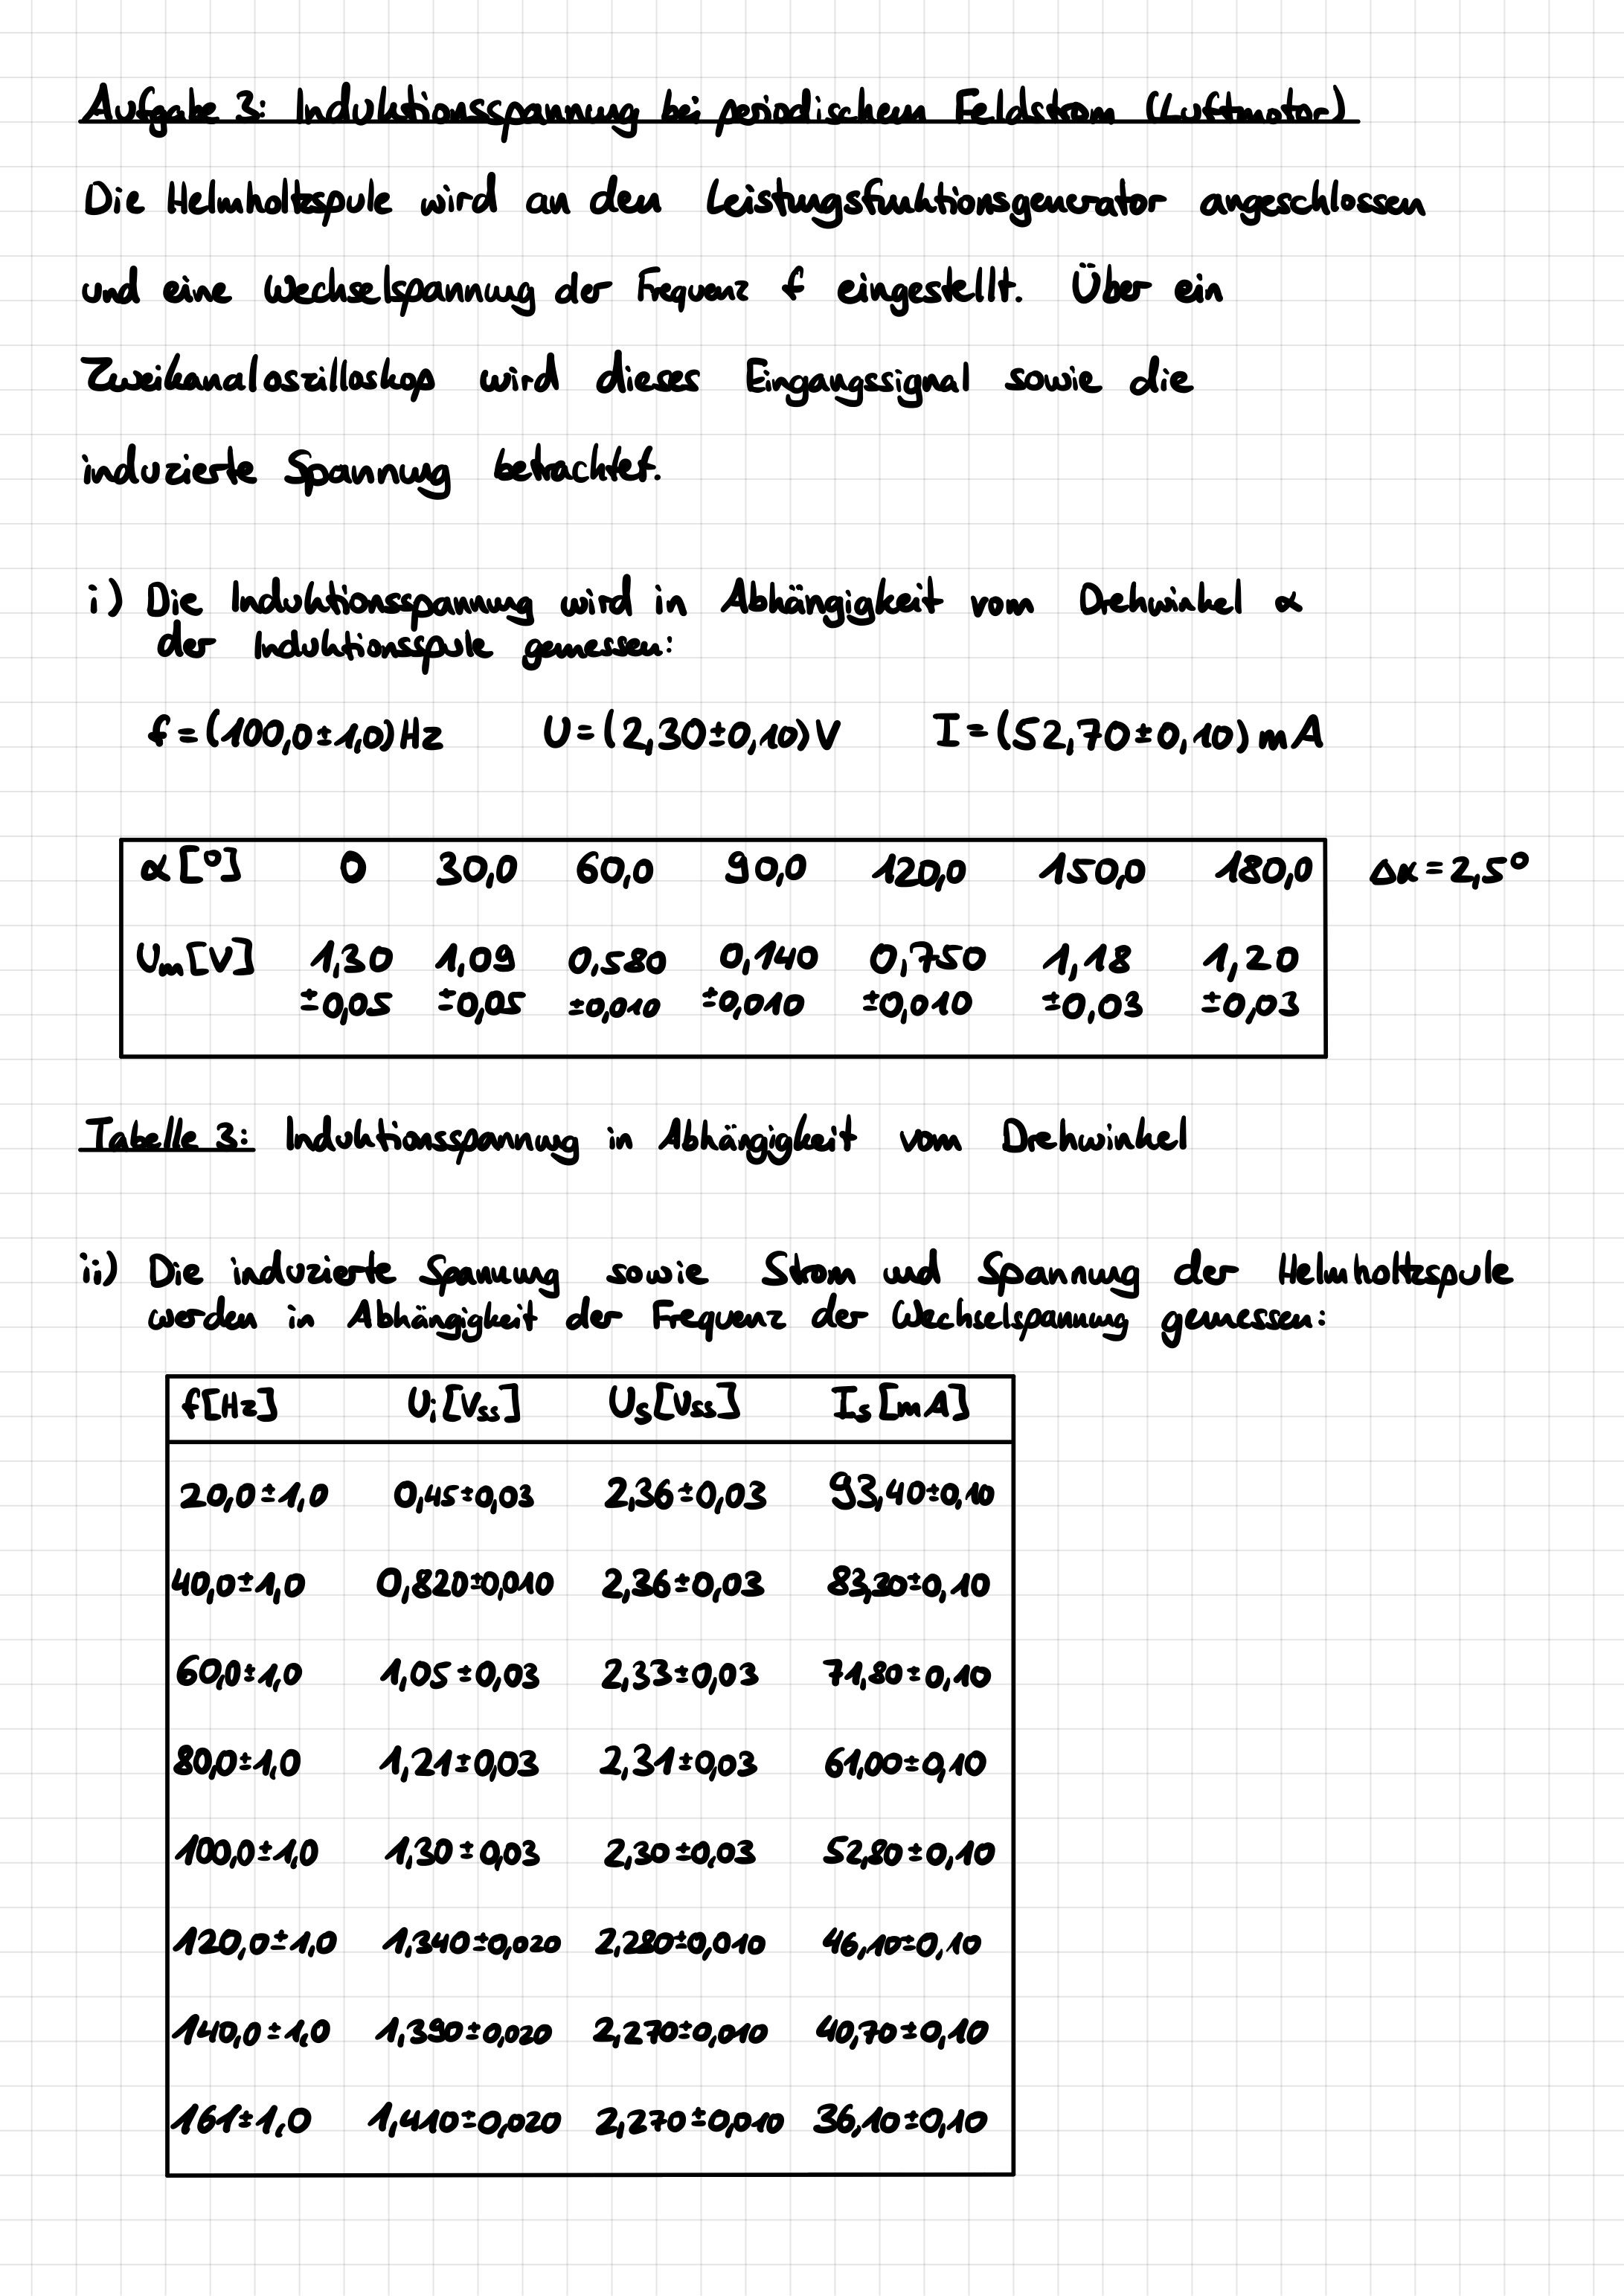
\includegraphics[width=\textwidth]{graphics/mess4.jpg}
\newpage
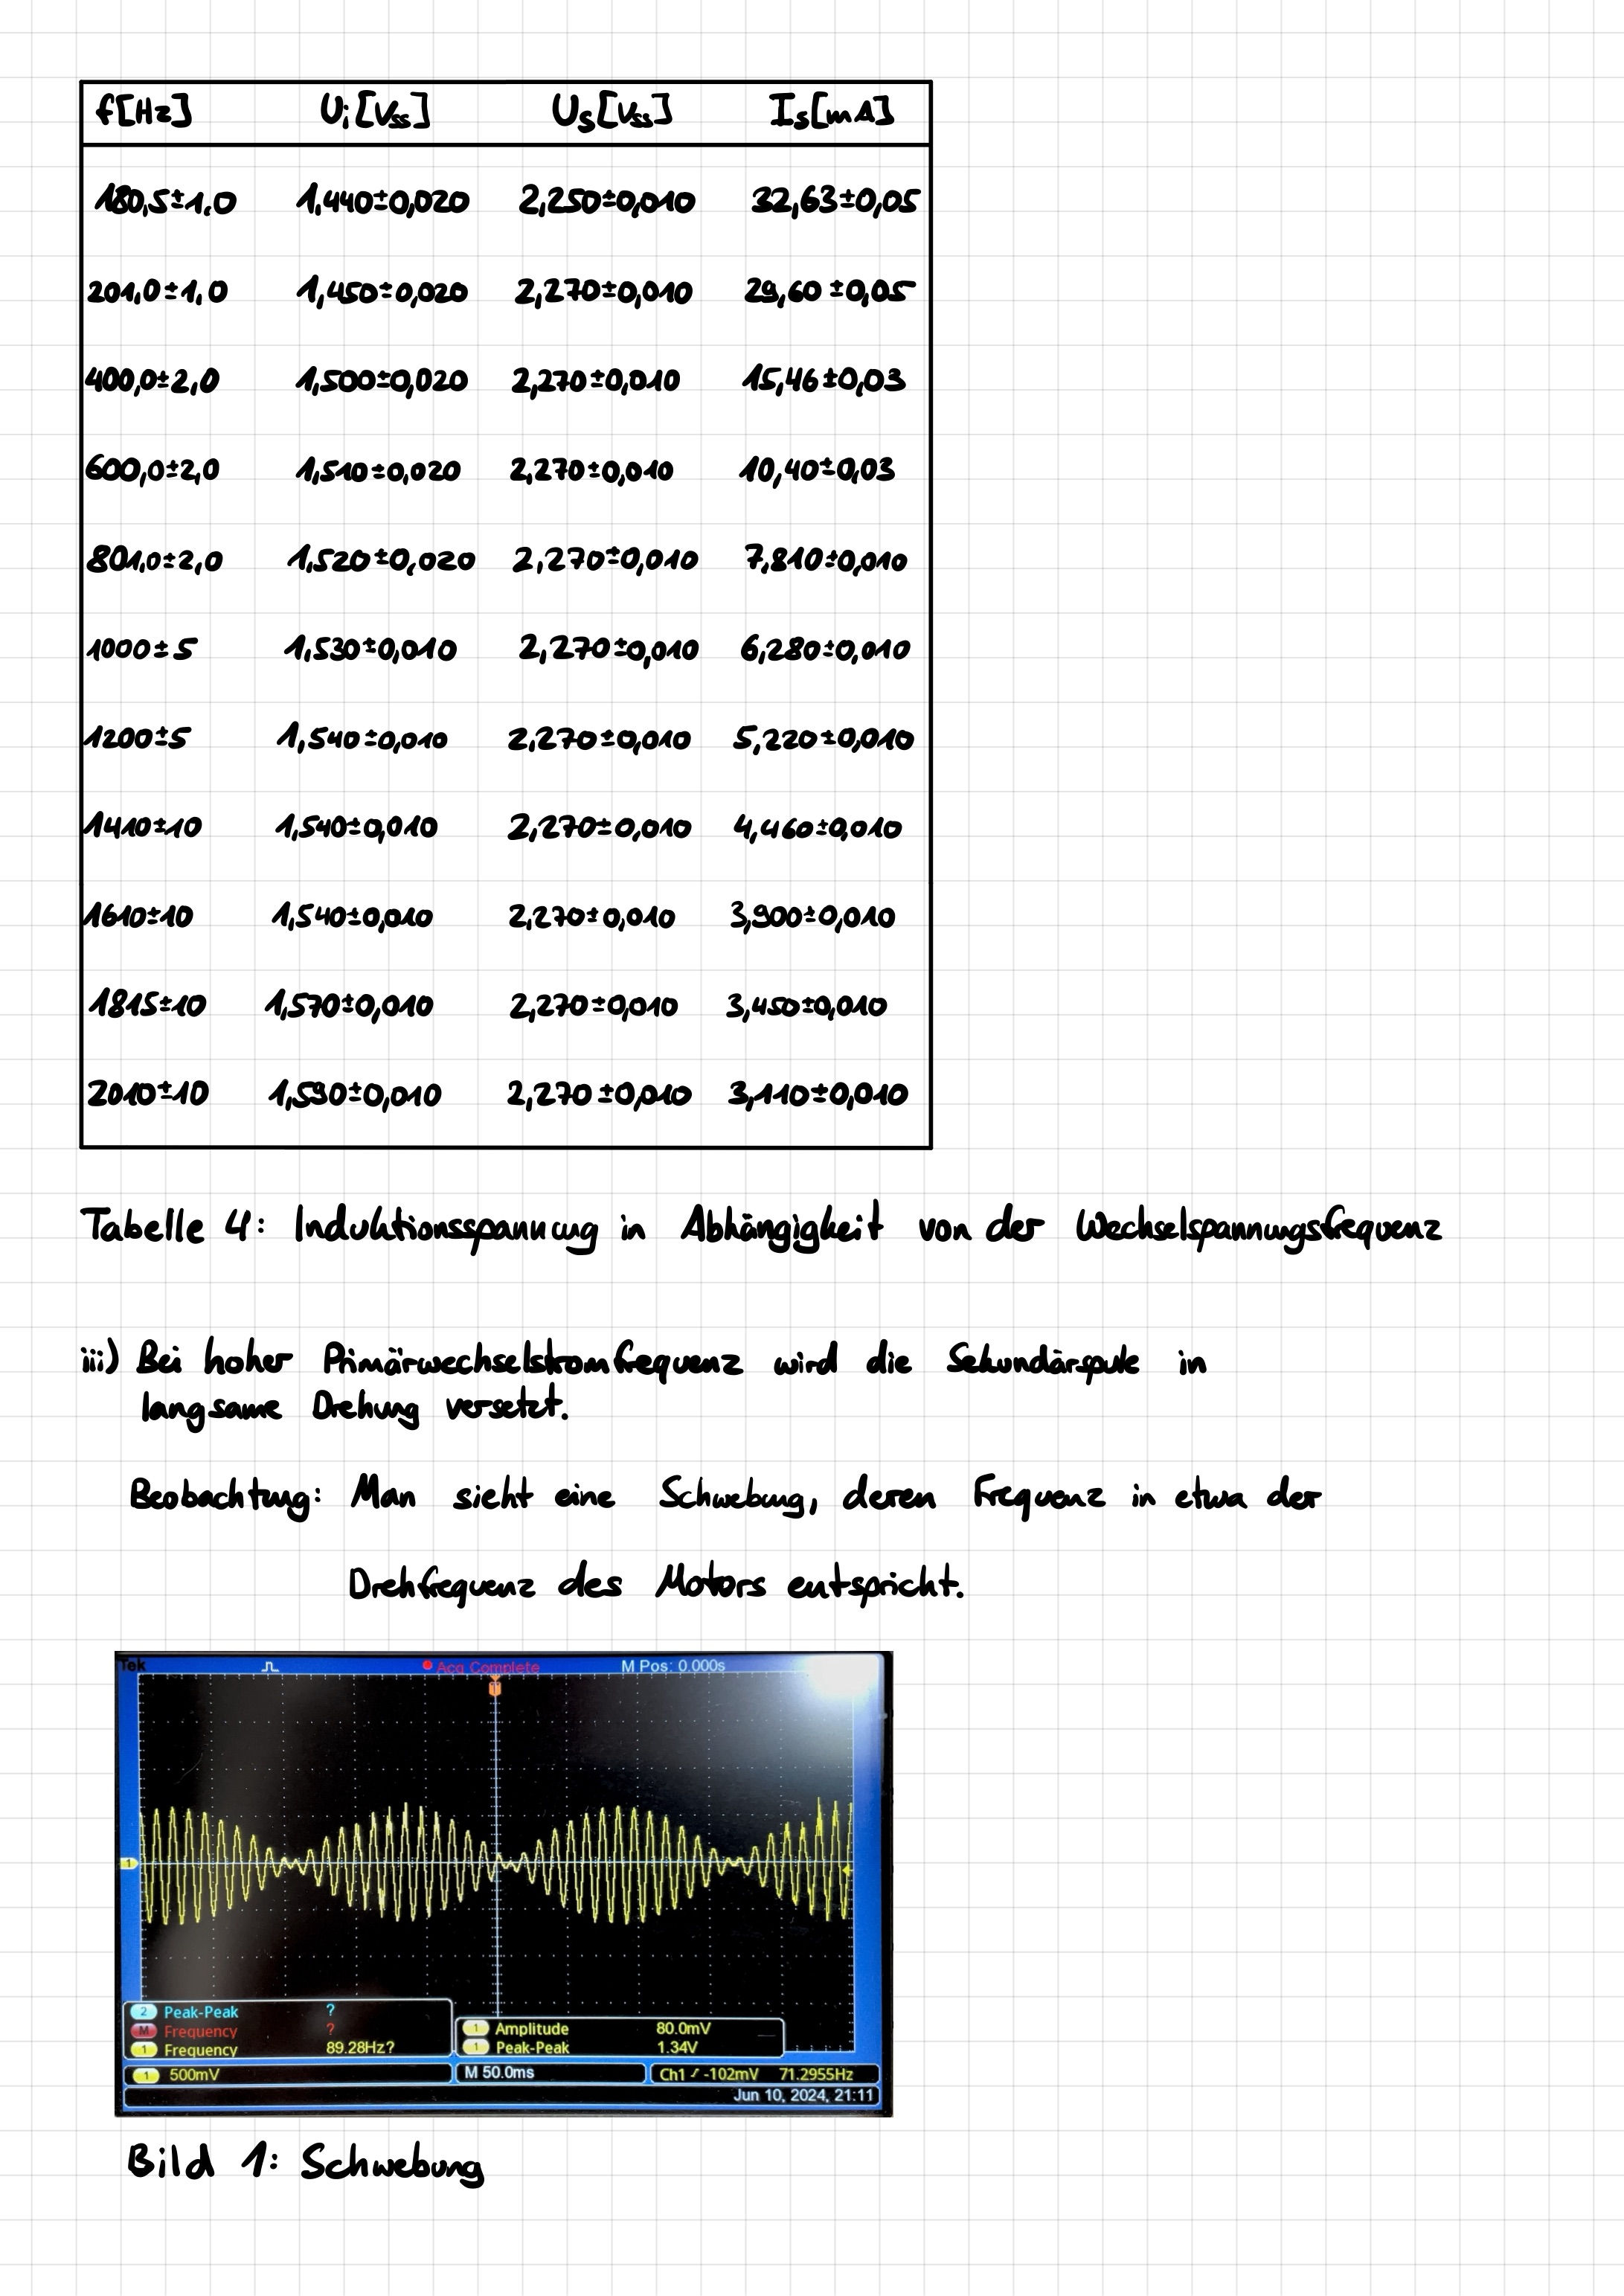
\includegraphics[width=\textwidth]{graphics/mess5.jpg}
\newpage
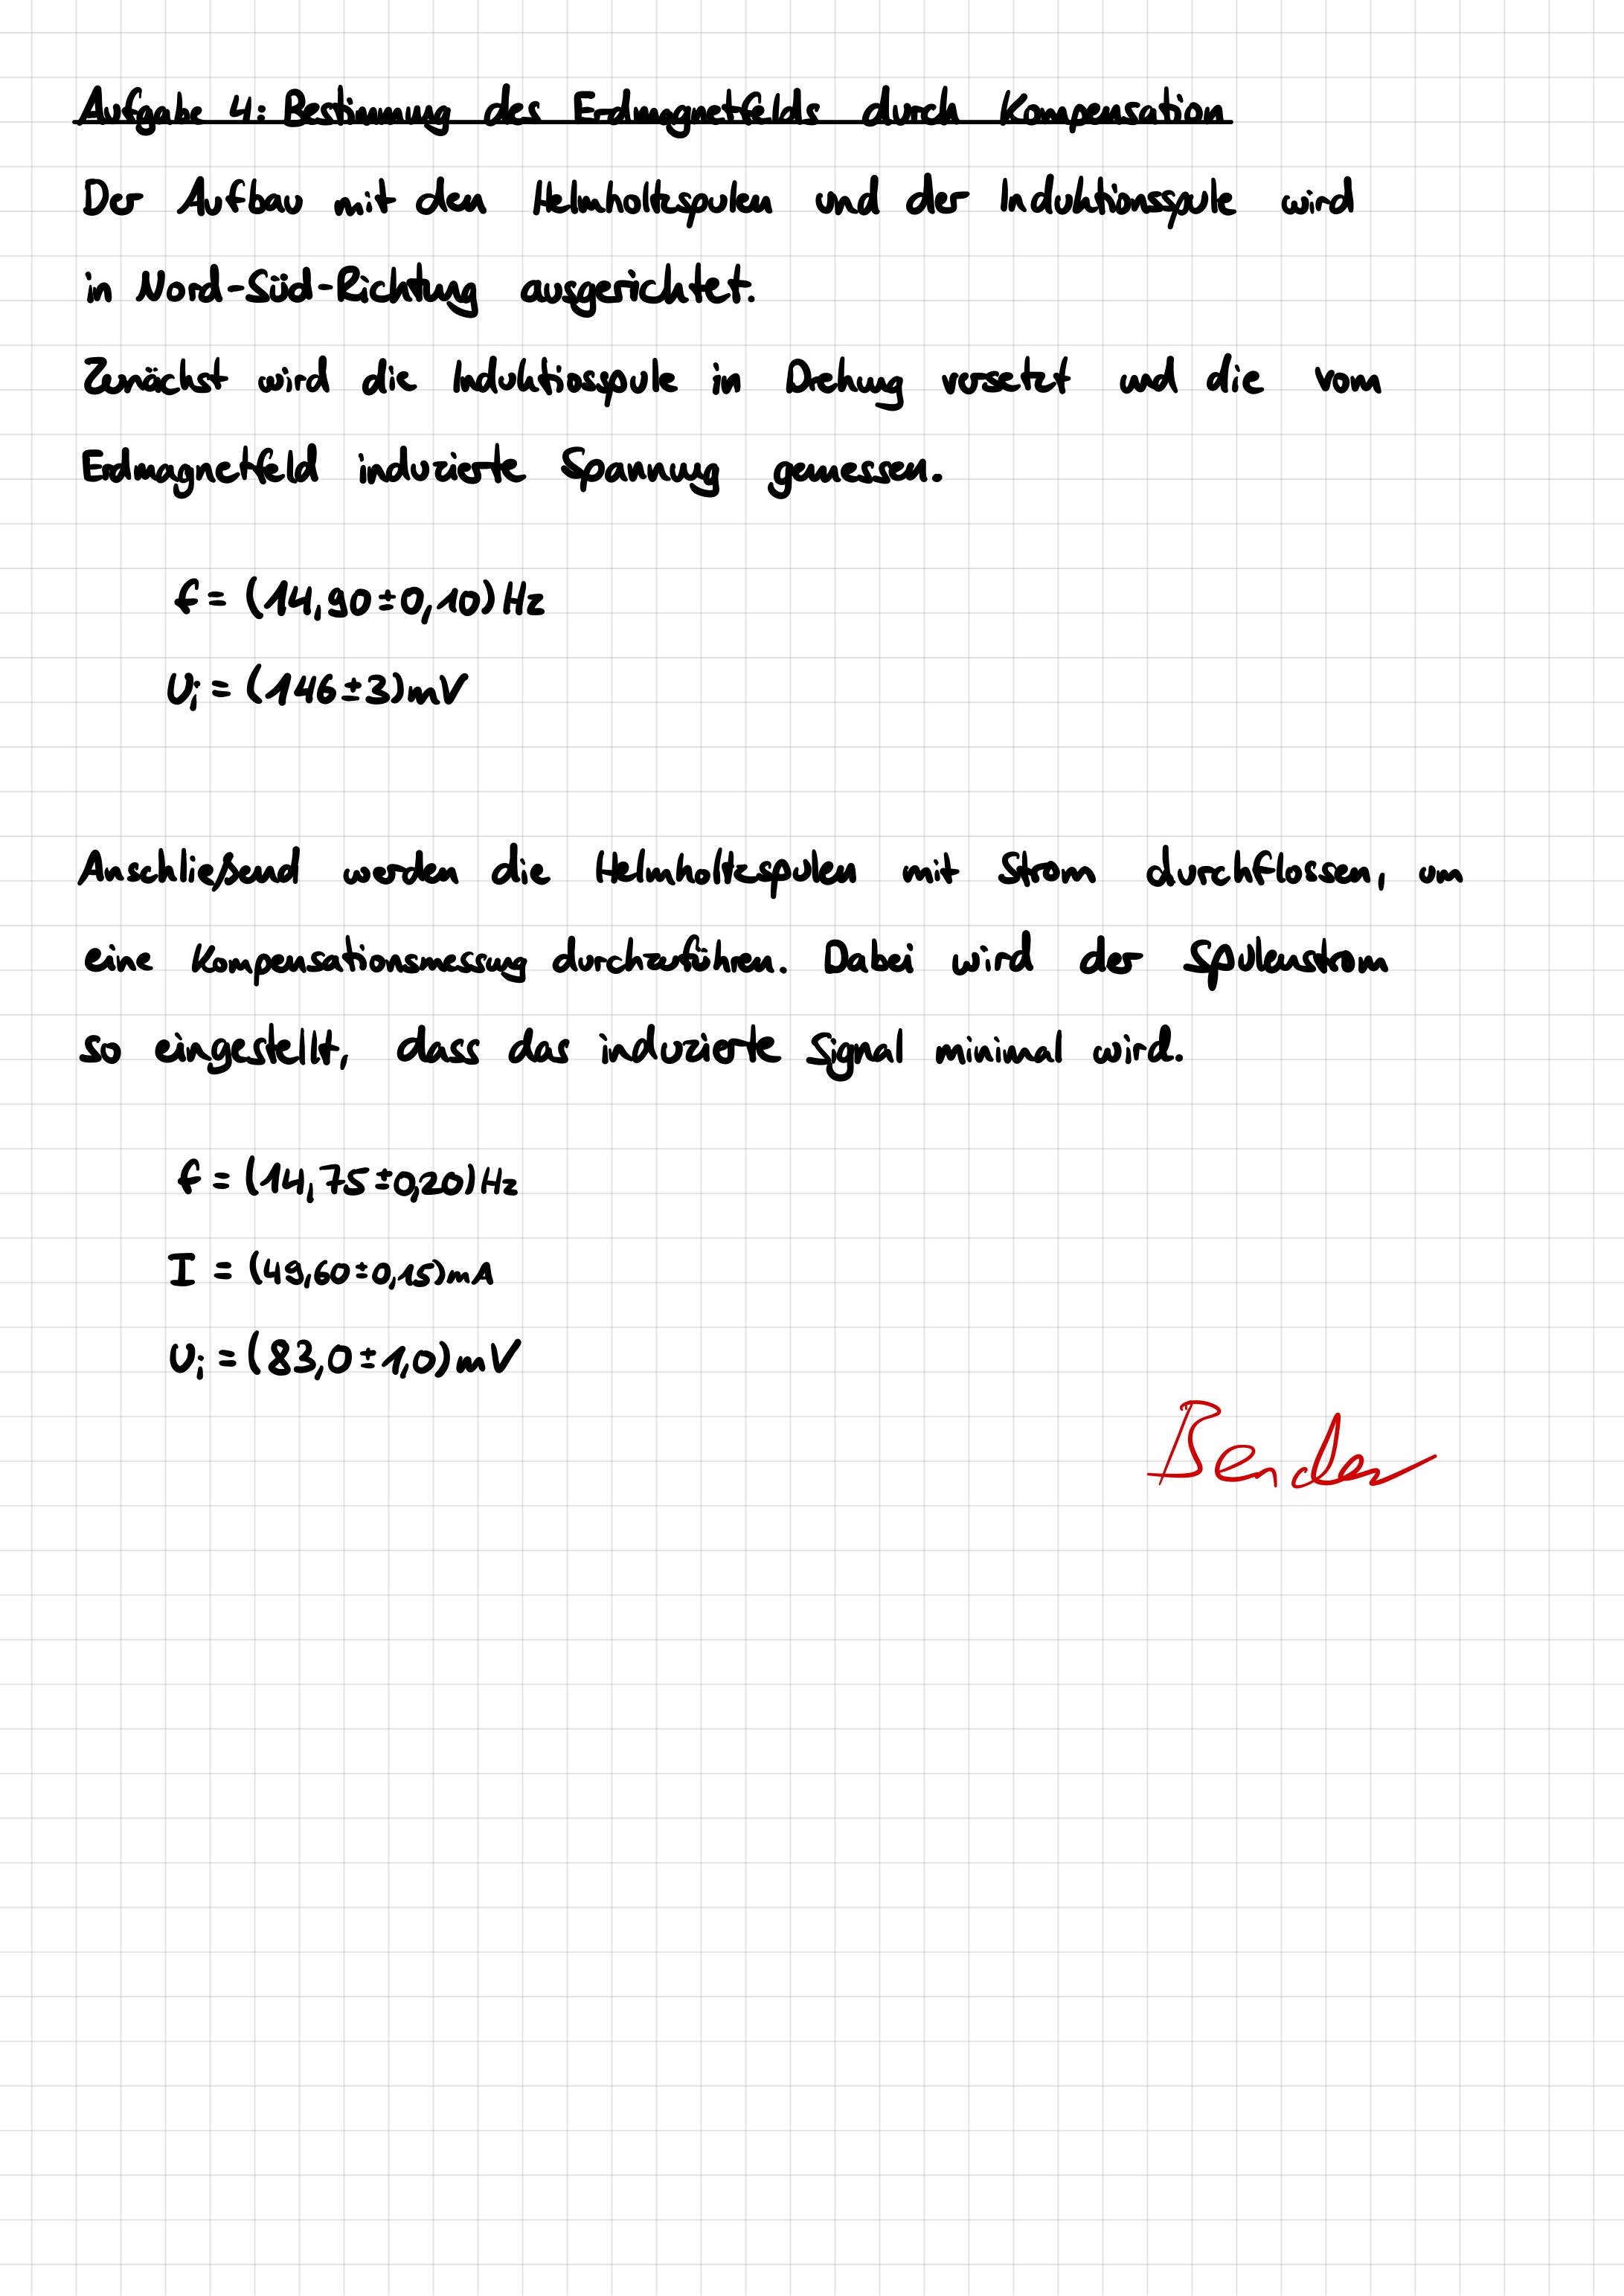
\includegraphics[width=\textwidth]{graphics/mess6.jpg}
\label{page:Schwebung}
\newpage

\addtocounter{table}{4}




\clearpage
\newpage
%-------------------------AUSWERTUNG-------------------------
\section{Auswertung}

In dieser Evaluation werden alle Fehler, sofern keine spezifische Angabe gemacht wird, mithilfe der Gauss'schen Fehlerfortpflanzung berechnet. Dies bedeutet, dass ein Wert $F$, der mit der Formel $f(a_1, ..., a_n)$ berechnet wird, den Fehler $\Delta F$ annimmt:

\begin{equation}
    \Delta F = \sqrt{\sum_n \left( \frac{\partial f}{\partial a_n} \cdot \Delta a_n \right)^2}.
\end{equation}

Des Weiteren erfolgen Signifikanztests von zwei Werten $a$ und $a'$ über die folgende Formel:

\begin{equation}
    \sigma = \frac{|a-a'|}{\sqrt{(\Delta a)^2 + (\Delta a')^2}}.
\end{equation}

Die Auswertung sowie Berechnung erfolgen über das dem Dokument angehängte Python-Programm. Hierbei erfolgen Fits von Funktionen mithilfe der 'curve\_fit'-Funktion des 'SciPy'-Packages und Plots werden mit 'matplotlib' erstellt.


\newpage
\subsection{Kommentar zum Vorversuch}

Zunächst wurde qualitativ beobachtet, wie ein Stabmagnet, der durch eine Spule bewegt wird, einen Strom in dieser erzeugt. Zunächst wurde der Magnet durch die Spule bewegt, danach die Spule um den Magnet bewegt. Dabei wurde beide male beobachtet, wie eine Spannung in der Spule induziert wird. Die beiden Fälle sind zudem völlig äquivalent, da nur die Relativbewegung von Spule zu Magnet relevant ist und es somit egal ist, ob sich der Magnet oder die Spule relativ zum anderen bewegt.

\subsection{Bestimmung des Magnetfelds der Helmholtz-Spule}

Wir beginnen, indem wir die in den Tabellen 1 und 2 des Messprotokolls aufgenommenen Induktionsspannungen separat in ein Diagramm als Funktion der Drehfrequenz beziehungsweise dem eingestellten Strom auftragen. An die Messwerte fitten wir Geraden an, zu sehen in den Abbildungen \ref{fig:A2-U(f)} \& \ref{fig:A2-U(I)}. Aus der Steigung der Geraden im $U(f)$-Diagramm $\alpha = (0,755 \pm 0,018)V_{SS}$/Hz berechnen wir gemäß Gleichung \ref{eq:Induktionsgesetz_Helmholtz} das Magnetfeld $B$, wobei $\alpha = U / f = 2 \pi \cdot U / \omega$ und der Sinus aufgrund der Amplitudenmessung gleich dem maximalen Wert 1 gesetzt wird. Ebenso wird berücksichtigt, dass die gemessene Spannung die Spitze-Spitze-Spannung ist, weshalb wir für die absolute Amplitude nochmal durch 2 teilen müssen und das Minuszeichen wird weggelassen. Somit erhalten wir: 

\begin{equation}
    \begin{split}
        B_{exp} &= \frac{\alpha}{4 \pi N A}, \\
        \Rightarrow \Delta B_{exp} &= B_{exp} \sqrt{\left( \frac{\Delta \alpha}{\alpha} \right)^2}, \\ \\
        &\Rightarrow \bm{B_{exp} = (360 \pm 9)\cdot 10^{-5}} \textbf{T}.
    \end{split}
\end{equation}

Hierbei wurden die gegebenen Werte der Induktionsspule $N_I = 4000$ und $A_I = 41,7 \cdot 10^{-4}$m$^2$ verwendet. Zum Vergleich berechnen wir den theoretischen Wert des Magnetfelds gemäß Gleichung \ref{eq:Magnetfeld_THEO}, wobei $N_H = 124$ und $r_H = 0,147$m der Helmholtz-Spule sowie der eingestellte Strom $I = (4,00 \pm 0,10)$A verwendet werden. Wir erhalten somit den folgenden theoretischen Wert:

\begin{equation}
    \bm{B_{theo} = (303 \pm 8)\cdot 10^{-5}} \textbf{T}.
\end{equation}

Der Vergleich der beiden Werte ergibt eine Sigmaabweichung von $4,94 \sigma$, was eine signifikante Abweichung darstellt. Ursachen hierfür könnten weitere nicht berücksichtigte Magnetfeldquellen im Raum, wie die Experimente der anderen Teilnehmer oder das Erdmagnetfeld, oder Schwankungen im eingestelltem Strom sowie der Rotationsfrequenz sein.  

\begin{figure}[!h]
    \centering
    \resizebox{0.8\textwidth}{!}{
    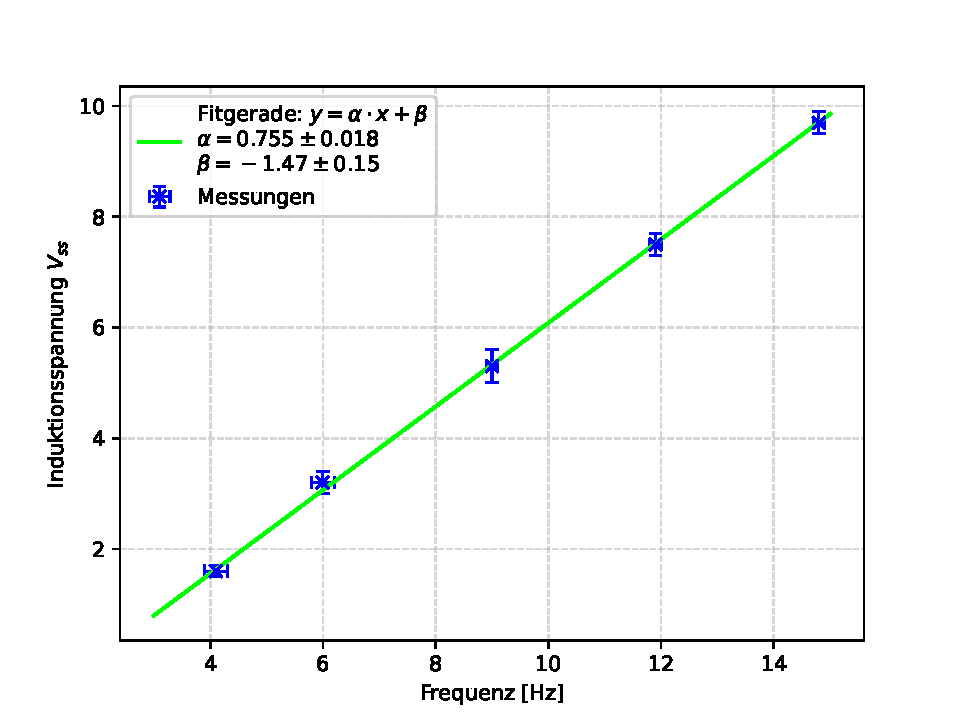
\includegraphics{plots/Induktionsgesetz_U(f).pdf}}
    \caption{A2 - Induktionsspannung $U(f)$}
    \label{fig:A2-U(f)}
\end{figure}

\begin{figure}[!h]
    \centering
    \resizebox{0.8\textwidth}{!}{
    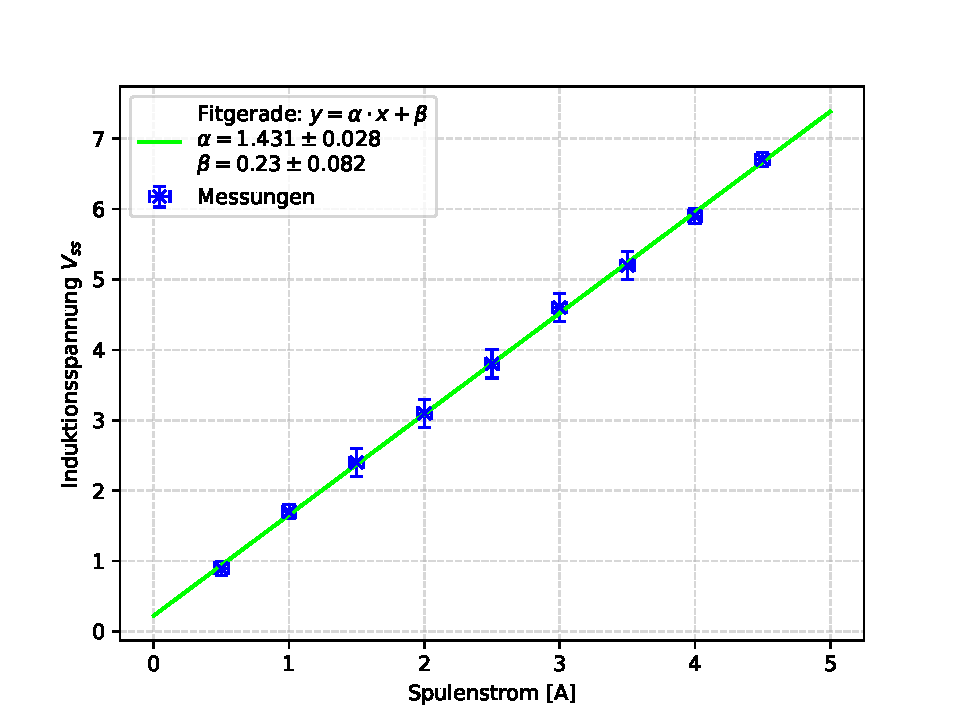
\includegraphics{plots/Induktionsgesetz_U(I).pdf}}
    \caption{A2 - Induktionsspannung $U(I)$}
    \label{fig:A2-U(I)}
\end{figure}

\clearpage
\newpage

\subsection{Wechselstrommessungen und Induktivität}

\subsubsection{Winkelabhängigkeit der Induktionsspannung}

Zunächst tragen wir die gemessene Spannung als Funktion des Winkels aus Tabelle 3 in ein Diagramm eintragen. Zur besseren qualitativen Analyse fitten wir die folgende absolute Cosinus-Funktion an, wobei $f$ die gemessene Frequenz und $A$ eine allgemeine Amplitude ist: 

\begin{equation}
    y = A |2 \pi N_I A_I f \cos{x}| + bkg.
\end{equation}

Der in Abbildung \ref{fig:A3-U(alpha)} dargestellte Plot zeigt das erwartete Verhalten. Bei 90° wird fast keine Spannung mehr induziert, da die Spule nun parallel zum Magnetfeld verläuft. Die verbleibende gemessene Spannung, welche für die Amplitude wieder halbiert werden muss, ist sehr klein und somit auf leichte Abweichungen des eingestellten Winkels sowie störende externe Magnetfelder zurückzuführen. Ebenso lässt sich beobachten, wie bei sich einer Umdrehung von 180° das gemessene Signal wie erwartet dem Signal bei 0° annähert, was auf die Symmetrie der beiden Fälle zurückzuführen ist. 

\begin{figure}[!b]
    \centering
    \resizebox{0.9\textwidth}{!}{
    \includegraphics{plots/Winkelabhängigkeit.pdf}}
    \caption{A3 - Winkelabhängigkeit der Induktionsspannung $U(\alpha)$}
    \label{fig:A3-U(alpha)}
\end{figure}

\newpage
\subsubsection{Abhängigkeit der Frequenz des Wechselstroms}

Wir stellen nun das Verhältnis der in Tabelle 4 gemessenen induzierten und angelegten Spannung $U_i / U_s$ als Funktion der Wechselstromfrequenz dar, Abbildung \ref{fig:A3-U(f)}. Deutlich zu erkennen ist die Abflachung mit resultierendem Plateau-Bereich oberhalb einer Frequenz von etwa 250Hz. Grund hierfür ist die verwendete Versuchsanordnung und der Fakt, dass es sich bei dem verwendeten Transformator um einen Lufttransformator handelt.

\begin{figure}[!h]
    \centering
    \resizebox{0.9\textwidth}{!}{
    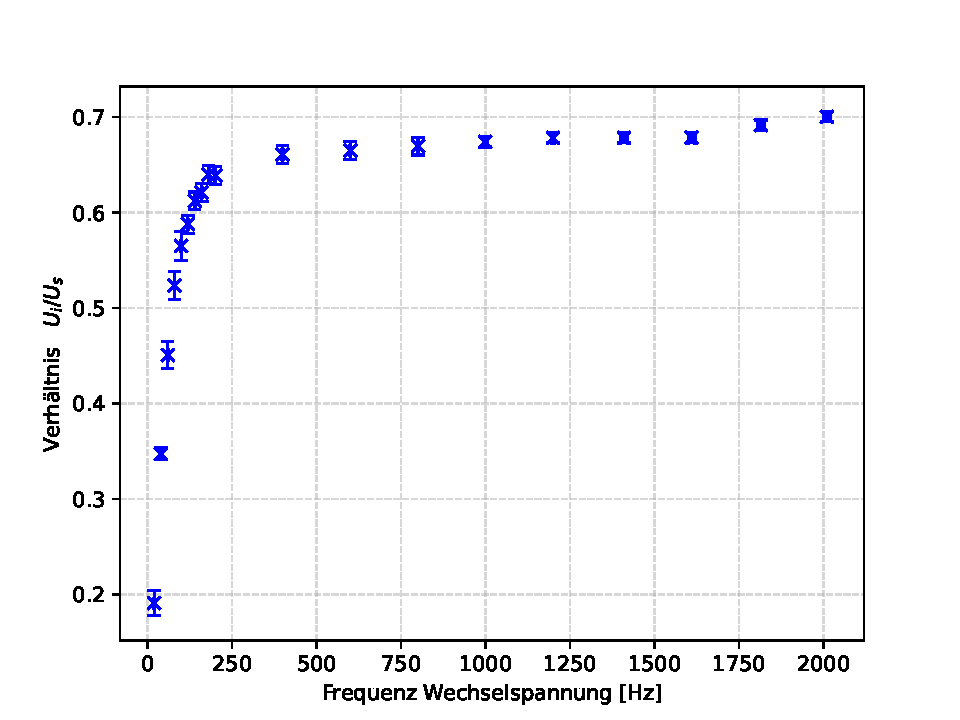
\includegraphics{plots/Wechselspannung-Frequenzabh.pdf}}
    \caption{A3 - Verhältnis der induzierten zur angelegten Spannung als Funktion der Wechselspannungsfrequenz}
    \label{fig:A3-U(f)}
\end{figure}


\newpage
\subsubsection{Induktivität der Helmholtz-Spule}

Um die Induktivität zu bestimmen, berechnen wir zunächst den Widerstand der Helmholtz-Spule, indem wir gemäß $U = I \cdot R$ die gemessenen Spannungen $U_S$ durch den Strom $I_S$ teilen. Diesen Widerstand plotten wir als Funktion der Wechselstromfrequenz und machen einen linearen Fit, zu sehen in Abbildung \ref{fig:A3-R(f)}. Aus der Steigung der Fitgeraden $\alpha = (0,3455 \pm 0,0007) \Omega /$Hz lässt sich gemäß Gleichung \ref{eq:Induktivität} die Induktivität bestimmen:

\begin{equation}
    \begin{split}
        L &= \frac{\alpha}{2 \pi}, \\
        \Rightarrow \Delta L&= \frac{\Delta \alpha}{2 \pi}, \\ \\
        &\Rightarrow \bm{L = (54,99 \pm 0,10)\cdot 10^{-3}} \textbf{H}.
    \end{split}
\end{equation}

\begin{figure}[!h]
    \centering
    \resizebox{0.9\textwidth}{!}{
    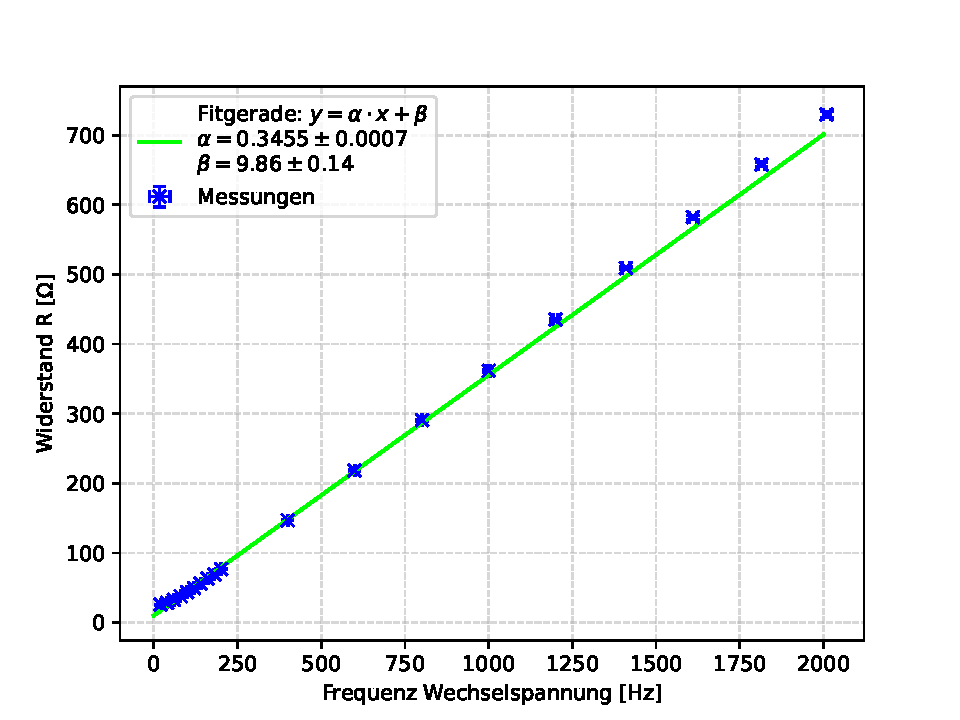
\includegraphics{plots/Widerstand-R(f).pdf}}
    \caption{A3 - Widerstand der Helmholtz-Spule R(f)}
    \label{fig:A3-R(f)}
\end{figure}

\newpage
\subsubsection{Kommentar zur beobachteten Schwebung}

Zuletzt wurde in diesem Versuchsteil zusätzlich zu einer anliegenden Wechselspannung auf der Helmholtz-Spule die Sekundärspule in eine langsame Drehung versetzt. Hierbei konnte, wie in Bild 1 des Messprotokolls gut zu erkennen, die erwünschte Schwebung beobachtet werden. Die Frequenz der innenliegenden Schwingungen ist hierbei gegeben durch den Wechselstrom und die einhüllende Welle entsteht durch die zusätzliche Drehung der Spule. Diese beiden Frequenzen addieren sich zu der beobachteten Schwebung.

\phantom{.}

\begin{figure}[!h]
    \centering
    \resizebox{0.9\textwidth}{!}{
    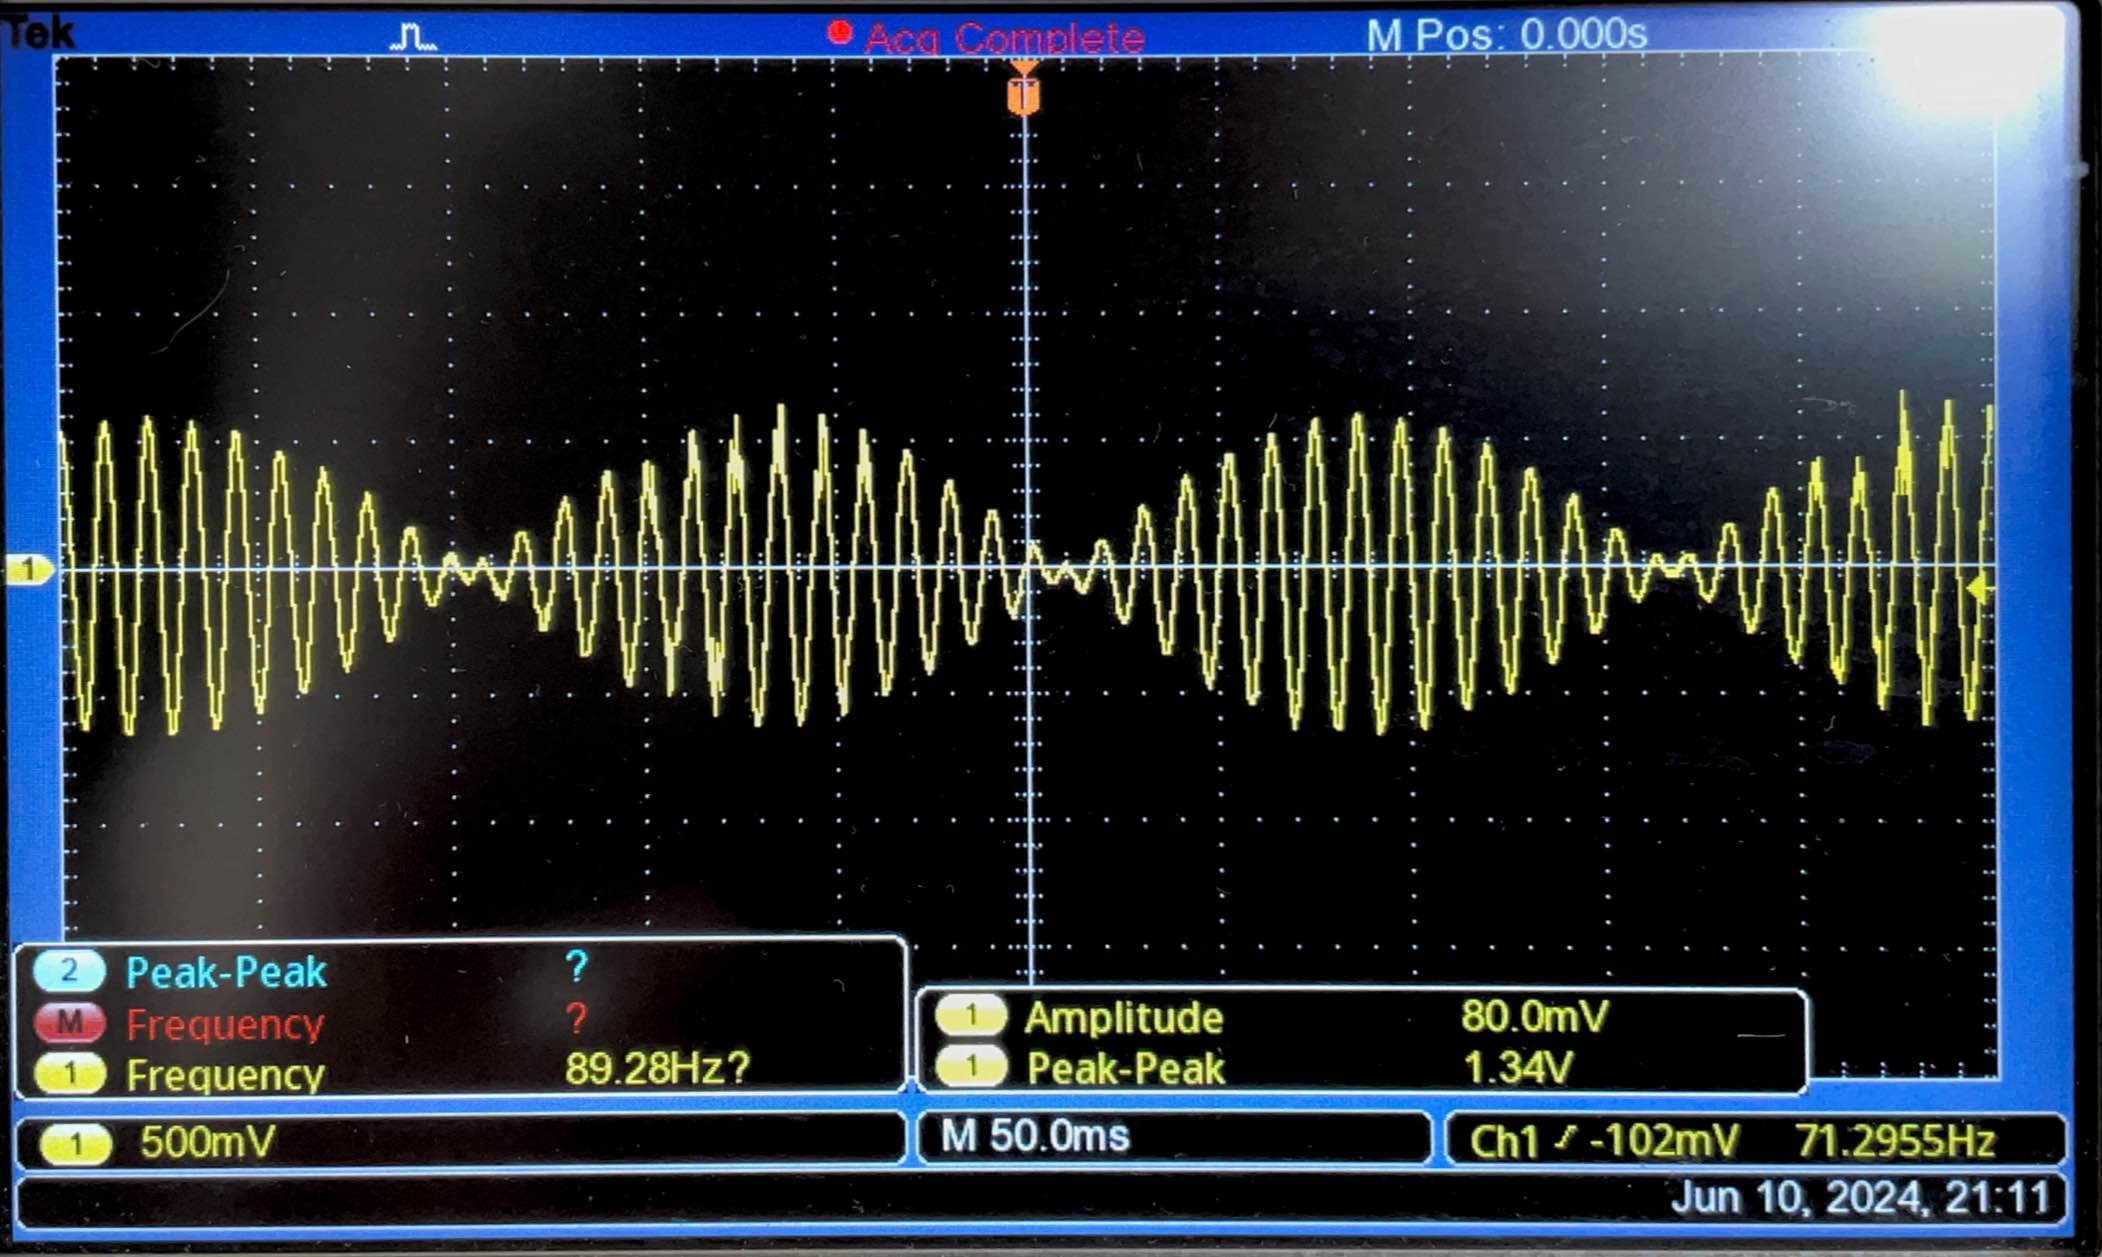
\includegraphics{graphics/Schwebung.jpg}}
    \caption{A3 - Aufgenommene Schwebung, siehe \hyperref[page:Schwebung]{Messprotokoll}}
    \label{fig:A3-Schwebung}
\end{figure}

\newpage
\subsection{Bestimmung des Erdmagnetfelds}

Wir beginnen mit der Messung ohne Kompensation und bestimmen aus der gemessenen Frequenz sowie Induktionsspannung das Erdmagnetfeld. Dazu verwenden wir erneut Gleichung \ref{eq:Induktionsgesetz_Helmholtz} und erhalten:

\begin{equation}
    \begin{split}
        B_{earth,exp} &= \frac{U_I}{4 \pi N A f}, \\
        \Rightarrow \Delta B_{earth,exp} &= B_{exp} \sqrt{\left( \frac{\Delta U_I}{U_I} \right)^2 + \left( \frac{\Delta f}{f} \right)^2}, \\ \\
        &\Rightarrow \bm{B_{earth,exp} = (4,67 \pm 0,10)\cdot 10^{-5}} \textbf{T}.
    \end{split}
\end{equation}

Wir vergleichen mit dem gegebenen Literaturwert (siehe \hyperref[eq:Erdmagnetfeld-Theo]{Einleitung}) und erhalten eine Abweichung von $2,14\sigma$, was insignifikant ist.

Wir betrachten nun die Messwerte der Kompensationsmessung. Für die Vertikalkomponente verwenden wir Gleichung \ref{eq:Magnetfeld_THEO} mit dem gemessenen Kompensationsstrom $I = (49,60 \pm 0,15)$A und erhalten:

\begin{eqnarray}
    \begin{split}
        B_{\bot,exp} &= \mu_0 \frac{8N}{\sqrt{125} r} I, \\
        \Rightarrow \Delta B_{\bot,exp} &= B_{\bot,exp} \sqrt{\left( \frac{\Delta I}{I} \right)^2}, \\ \\
        &\Rightarrow \bm{B_{\bot,exp} = (3,762 \pm 0,011)\cdot 10^{-5}} \textbf{T}. 
    \end{split}
\end{eqnarray}

Die horizontale Komponente bestimmen wir aus der verbleibenden Restspannung analog zum Erdmagnetfeld ohne Kompensation und erhalten:

\begin{eqnarray}
    \bm{B_{\parallel,exp} = (2,68 \pm 0,05)\cdot 10^{-5}} \textbf{T}. 
\end{eqnarray}

Aus dem Literaturwerten des Magnetfelds und der Inklinination berechnen wir die theoretischen Werte für die horizontale und vertikale Komponente und erhalten:

\begin{equation}
    \begin{split}
        B_{\bot,theo} = 44399,2 \cdot 10^{-9} \text{T}, \\
        B_{\parallel,theo} = 20515,3 \cdot 10^{-9} \text{T}.
    \end{split}
\end{equation}

Somit erhalten wir Abweichungen von $59,58\sigma$ für die vertikale und $13,00\sigma$ für die horizontale Komponente. Diese Werte weisen enorme Abweichungen auf. Höchstwahrscheinlich wird die Hauptursache hierfür eine nicht exakte Kompensation sein, da das Einstellen des richtigen Stromwertes sehr inakkurat war und nie eine 100\%-ige Kompensation erzielt werden konnte. 

Da der horizontale Wert eine geringere Abweichung aufweist verwenden wir diesen zur Bestimmung der Inklination gemäß Gleichung \ref{eq:Inklination}. Wir verwenden den ohne Kompensationsmessung bestimmten Wert für den Betrag des Erdmagnetfelds und erhalten:

\begin{equation}
    \bm{i = (55,0 \pm 1,1)^\circ}.
\end{equation}

Verglichen mit dem Literaturwert ergibt sich eine Abweichung von $9,04\sigma$, was ebenfalls signifikant ist. Hier wird insbesondere die Ungenauigkeit des Werts der horizontalen Komponente für die hohe Abweichung gesorgt haben. 


\clearpage
\newpage
%---------------PRÄSENTATION DER ENDERGEBNISSE---------------
\section{Zusammenfassung der Endergebnisse}

In diesem Versuch wurde die Induktion mithilfe der Helmholtz-SPule untersucht. Zunächst machten wir die qualitative Beobachtung, dass bei einer Relativbewegung von einem Magnet durch eine Spule eine Spannung induziert wird. Mit diesem Prinzip bestimmten wir das Magnetfeld in der Helmholtz-Spule als

\begin{equation}
    B_{exp} = (360 \pm 9)\cdot 10^{-5} \text{T},
\end{equation}

was signifikant vom theoretischen Wert abweicht. Als Gründe wurden hier Störmagnetfelder und Stromschwankungen genannt. 

Anschließend betrachteten wir qualitativ die Winkel- und Wechselstromfrequenzabhängigkeit der induzierten Spannung, wobei beide Male erwartete Verläufe und Verhaltensweisen reproduziert werden konnten.

Ebenso berechneten wir die Induktivität der Helmholtz-Spule zu 

\begin{equation}
    L = (54,99 \pm 0,10)\cdot 10^{-3} \text{H}.
\end{equation}

Da hier kein Literaturwert existiert konnte kein quantitativer Vergleich erfolgen. 

Daraufhin betrachteten wir noch qualitativ die zu erwartende Schwebung bei gleichzeitigem Wechselstrombetrieb und separater Drehung der Sekundärspule, bevor wir uns dem letzten Versuchsteil des Erdmagnetfelds zuwendeten. Hier bestimmten wir zunächst den Betrag des Erdmagnetfelds und daraufhin die vertikale sowie horizontale Komponente:

\begin{equation}
    \begin{split}
        B_{earth,exp} &= (4,67 \pm 0,10)\cdot 10^{-5} \text{T}, \\
        B_{\bot,exp} &= (3,762 \pm 0,011)\cdot 10^{-5} \text{T}, \\
        B_{\parallel,exp} &= (2,68 \pm 0,05)\cdot 10^{-5} \text{T}.
    \end{split}
\end{equation}

Hierbei war beim Betrag keine signifikante Abweichung festzustellen, dafür aber wichen die beiden Komponenten stark von den Literaturwerten ab. Ebenso konnte die Inklination nur mit großer Abweichung bestimmt werden:

\begin{equation}
    i = (55,0 \pm 1,1)^\circ
\end{equation}


\newpage
%---------------ZUSAMMENFASSUNG UND DISKUSSION---------------
\section{Diskussion}

Wie in der Zusammenfassung deutlich zu erkennen ist, weisen viele der in diesem Versuch bestimmten Werte starke Abweichungen von den Literaturwerten auf. Die bereits genannten potenziellen Fehlerquellen werden hierbei die Hauptgründe gewesen sein. Insbesondere beim letzten Versuchsteil sind die Abweichungen so auffällig, dass ernsthaft an der Richtigkeit der Durchführung dieses Versuchsteils gezweifelt werden muss. Die bereits vermutete Hauptfehlerquelle der Kompensationseinstellung hätte mit digitaler Assistenz deutlich besser funktioniert, wie beispielsweise einem Programm, welches automatisch verschiedene Stromeinstellungen und deren Output testet, oder allein einer akkurateren digitalen anstatt analogen Einstellungsmöglichkeit der Stromstärke. Wie bereits erwähnt war nämlich keine 100\%-ige Kompensation möglich und es verblieb immer ein Restsignal bei jeder getesteten Einstellung. 

Ebenso lässt sich zum Aufbau generell noch sagen, dass die Riemenhalterung sowie der Riemen selbst, welcher benutzt wurde, um die Sekundärspule mit dem Drehmotor zu verbinden, bei unserem Versuchsaufbau beide etwas ungenau wirkten und eine Drehung erzeugten, deren Frequenz immerzu stark schwankte. Somit könnte auch hieraus eine große Varianz der Messwerte bei den relevanten Versuchsteilen resultieren. 

Abschließend lässt sich aber dennoch sagen, dass der Versuch trotz der nicht allzu zufriedenstellenden Ergebnisse dennoch eine interessante und lehrreiche Einführung in die Grundlagen der Induktion darstellt. 
 
\newpage
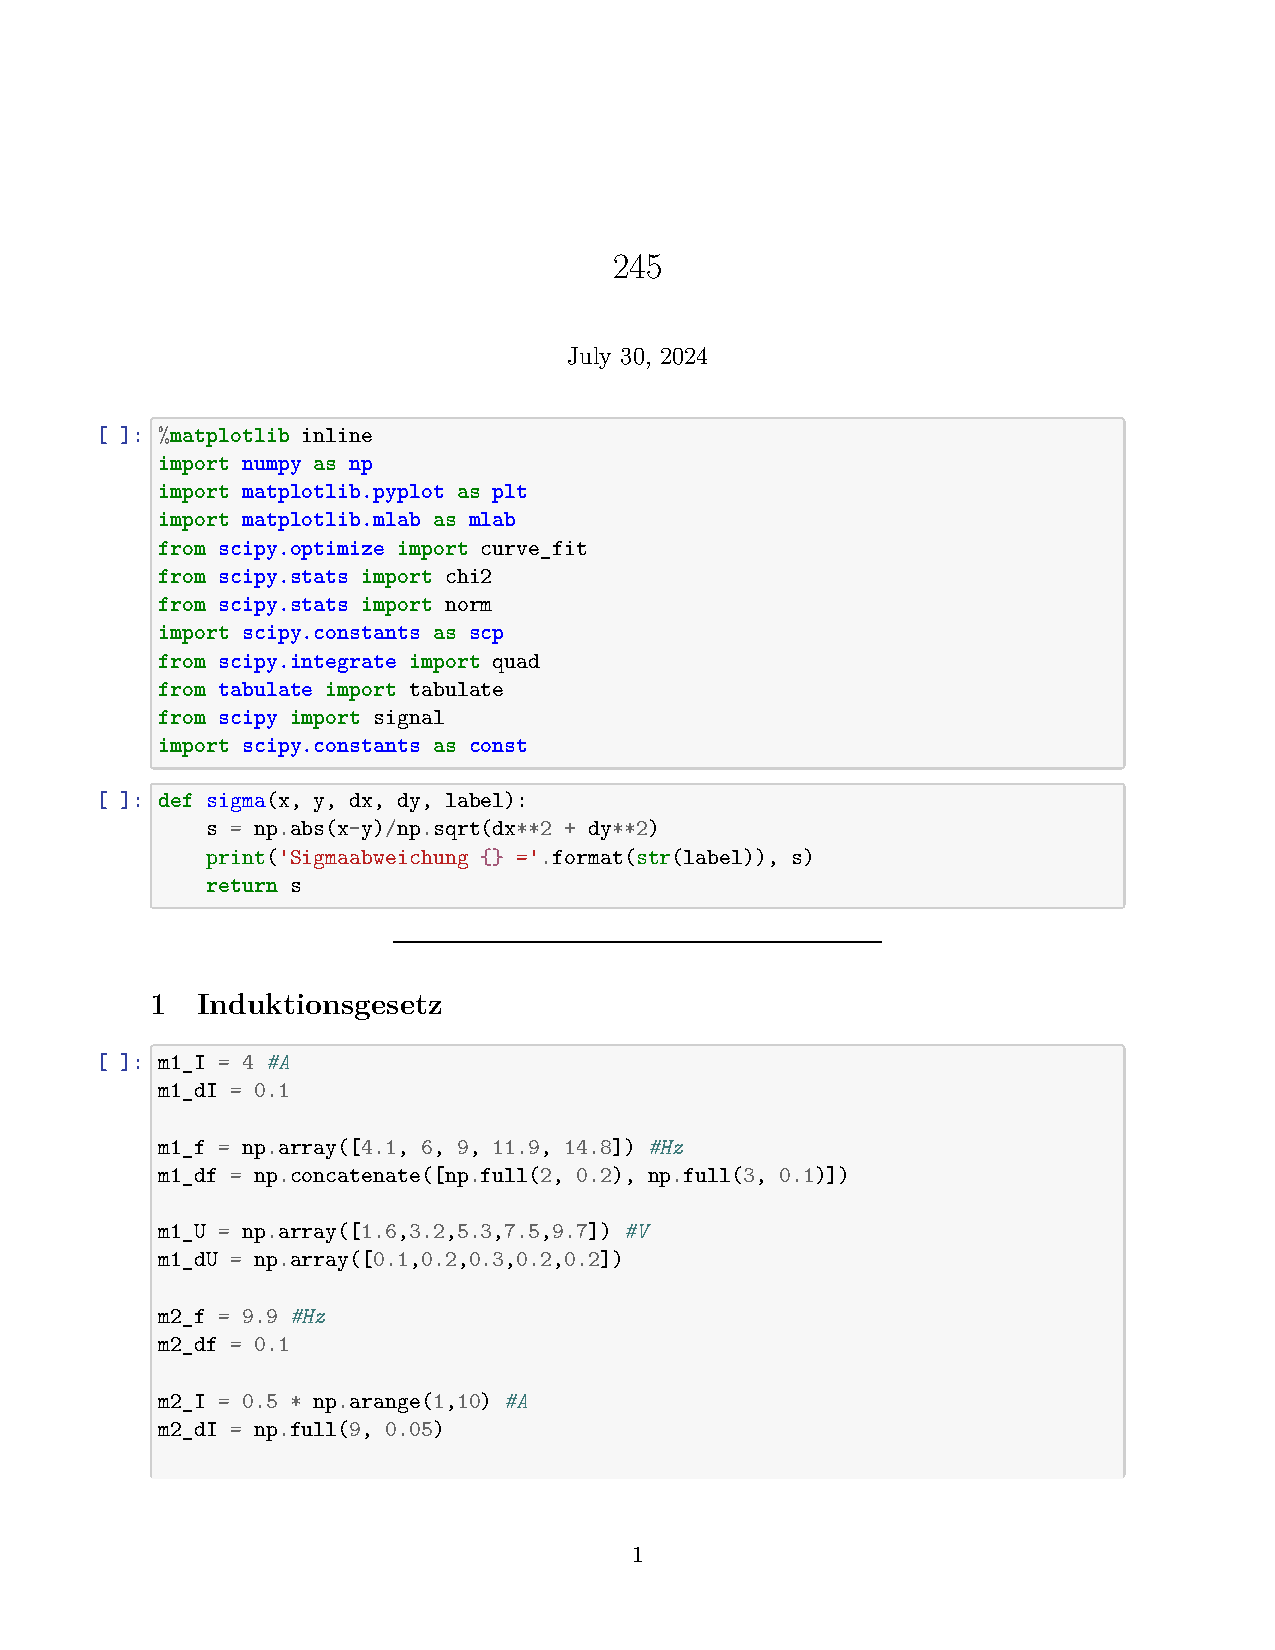
\includepdf[pagecommand=\invisiblesection{Python-Code},scale=0.8,pages=1]{245.pdf}
\includepdf[pagecommand={},scale=0.8,pages=2-last]{245.pdf}

\end{document}

